% 电子管收音机
% 电子管收音机.tex

\documentclass[12pt,UTF8]{ctexbook}

% 设置纸张信息。
\input{../../../common/page}

% 设置字体，并解决显示难检字问题。
\xeCJKsetup{AutoFallBack=true}
\setCJKfamilyfont{hei}{SimHei}
\setCJKfamilyfont{kai}{KaiTi}

% 设置支持西里尔字母的字体
\setmainfont{Times New Roman}
\setsansfont{Arial}
\setmonofont{Consolas}

% 目录 chapter 级别加点（.）。
\usepackage{titletoc}
\titlecontents{chapter}[0pt]{\vspace{3mm}\bf\addvspace{2pt}\filright}{\contentspush{\thecontentslabel\hspace{0.8em}}}{}{\titlerule*[8pt]{.}\contentspage}

% 支持目录点击跳转
\usepackage[colorlinks,linkcolor=blue,citecolor=blue,urlcolor=blue]{hyperref}

% 设置 part 和 chapter 标题格式。
\ctexset{
	part/name= {第,卷},
	part/number={\chinese{part}},
	chapter/name={第,章},
	chapter/number={\arabic{chapter}}
}

% 图片相关设置。
\usepackage{graphicx}
\usepackage{float}
\graphicspath{{Images/}}

% 设置署名格式。
\newenvironment{shuming}{\hfill\zihao{4}}

% 注脚每页重新编号，避免编号过大。
\usepackage[perpage]{footmisc}

% 设置古文原文格式。
\newenvironment{yuanwen}{\bfseries\zihao{4}}

% 设置段落间距
\setlength{\parskip}{0.8em plus 0.2em minus 0.1em}

% 列表格式支持，列表项向右偏移。
\usepackage{enumitem}

% 数学公式支持
\usepackage{amsmath}

\title{\heiti\zihao{0} 电子管收音机}
\author{WangFei}
\date{\today}

\begin{document}

\maketitle
\tableofcontents

\frontmatter
\chapter{前言}

矿石收音机虽有其独特魅力，但其核心的矿石检波器灵敏度低且稳定性差，需要用细针在矿石表面仔细寻找灵敏点。如今我们制作矿石收音机时，通常用晶体二极管替代矿石检波器，但晶体二极管是半导体技术成熟后的产物，比矿石检波器晚出现数十年。在电子管诞生初期，人们只能依赖这种需要精心调试的矿石检波器。为了寻求更可靠的无线电信号检测方法，研究人员从电灯泡中获得了灵感。

\mainmatter

\part{真空二极管的诞生}

\chapter{从静电场到热电子发射}

\section{静电场的基本原理}

我们知道，在两个金属板之间加上直流电压，板间就会建立起静电场。如下图所示：

\begin{figure}[htbp]
    \centering
    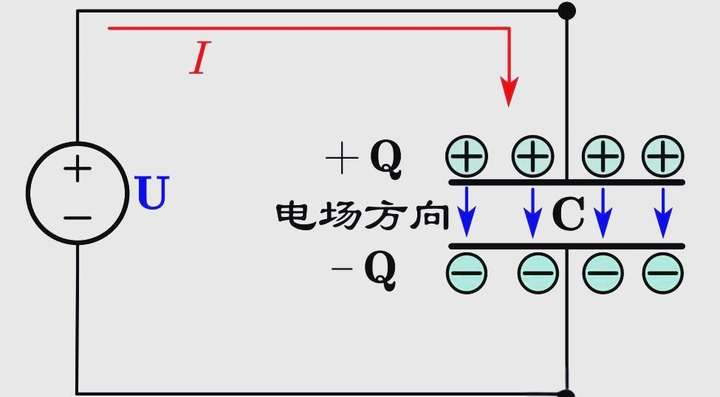
\includegraphics[width=0.7\linewidth]{electrostatic_field.jpg}
    \caption{平行金属板间的静电场}
    \label{fig:electrostatic_field}
\end{figure}

\section{热电子发射现象}

与此同时，物理学家还发现，当金属被加热到炽热状态时，它的表面会向外释放电子，这就是\textbf{热电子发射}，也叫\textbf{爱迪生效应}。

于是人们想到：如果将这两种现象结合会怎样？将平行金属板的负极替换为通电加热的灯丝，使其发射电子；正极板则保持静止等待接收电子。

整个装置要怎样保护？为了避免灯丝在空气中瞬间烧毁，也为了让飞出的电子不会撞上空气分子而散乱，人们把灯丝和金属板一起封进一个抽成高度真空的玻璃泡里。于是，\textbf{真空二极管}诞生了。

\section{电子管的真空度}

电子管内必须保持高度真空，不允许存在大量残余气体。如果残余气体过多，电子会与气体分子碰撞而降低运动速度，同时产生二次电子发射和气体电离，形成复杂的气体放电现象，干扰正常电子流。此外，残余气体会导致发射电子的电极氧化损坏。因此，电子管也被称为真空管。

电子管玻璃泡壁上常可见一层银色或黑色薄膜，这是抽空后利用吸气剂吸收残余气体留下的痕迹。吸气剂附着在电极后方的小金属杯或支架上，受热时与残余气体化合，形成这层薄膜。

\chapter{电子管的阴极结构}

根据释放电子的结构不同，电子管的阴极主要分为两种。

\section{直热式阴极}

第一种是\textbf{直热式阴极}：灯丝本身就是发射电子的阴极。通电后灯丝被加热至高温，电子直接从灯丝表面发射出来。这种结构简单直接，但由于灯丝同时承载加热电流，微小的电压波动会叠加在电子流上，容易引入交流哼声。

\section{旁热式阴极}

第二种是\textbf{旁热式阴极}。它将加热和发射功能分离：灯丝仅负责发热，外部套有涂覆特殊氧化物的金属圆筒，由圆筒发射电子。由于阴极与加热灯丝在电气上绝缘，阴极本身是等电位面，发射的电子流非常稳定，即使采用交流电加热也几乎没有干扰。后来绝大部分收音机和放大器使用的电子管都采用这种旁热式阴极。

\section{灯丝材料}

电子管的热电子发射来源于"灯丝"（又称丝极）。电流通过灯丝产生热量并发射电子。电子管常用的灯丝材料包括：

（1）\textbf{钨丝灯丝} 和普通电灯泡的灯丝一样用钨丝做成，坚固耐用，在2400°C时发射性能最好，但需要消耗较大的功率，所以不太经济。

（2）\textbf{钍层灯丝} 在钨里面加入一些氧化钍，经过特别处理之后，钨丝表面就覆盖一层薄钍膜，可以在较低的温度下发射大量电子。当1000°C时发射的电子，就和同面积的钨丝在2000°C时所发射的电子数量相等。不过在灯丝过热或电压过高时，钍层会损坏失效，不再发射电子。

（3）\textbf{碳化层灯丝} 是钍层灯丝经过萘蒸气或乙炔蒸气的热处理，在表面产生一层碳化钨，能够将钍层原子固定起来，不易蒸发，工作温度也只有1800°C。不过性质较脆，在经常移动的收音机中使用时，灯丝容易因振动而折断。

（4）\textbf{涂钍灯丝} 它是在钨丝外涂一层氧化铜，再涂一层钍而成。所需工作温度不高，发射效率也高，不会因过热而失效，是一种比较可靠的灯丝。

（5）\textbf{氧化层灯丝} 它是在铁镍合金（或其他化合物）制成的灯丝上，涂一层钡或锶的碳酸盐，在较低温度下（约650-850°C）就能发射大量电子，所以又叫做"活化灯丝"。性能比钍层灯丝更稳定，现在小型收音机中所用的电子管，绝大部分采用这种经济高效的活化灯丝。

\chapter{真空二极管的工作原理}

\section{二极管电子管的结构}

二极管电子管是一种最简单的电子管，它是在一个抽成真空的玻璃容器中装置两个电极——阴极和屏极。阴极是由一根金属丝或金属管子作成，在它表面涂有一层加热到一定温度就能发放出电子的氧化物薄层。

屏极（又称板极）是套在阴极外围的，由金属板作成的套筒。

\begin{figure}[htbp]
    \centering
    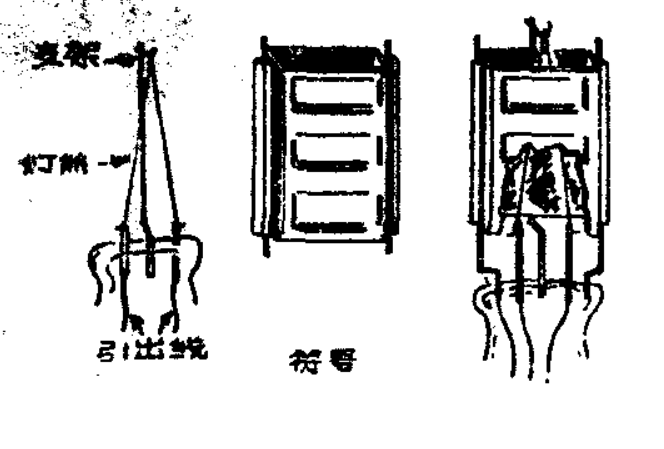
\includegraphics[width=0.7\linewidth]{diode_structure.png}
    \caption{二极管的构造}
    \label{fig:diode_structure}
\end{figure}

\begin{figure}[htbp]
    \centering
    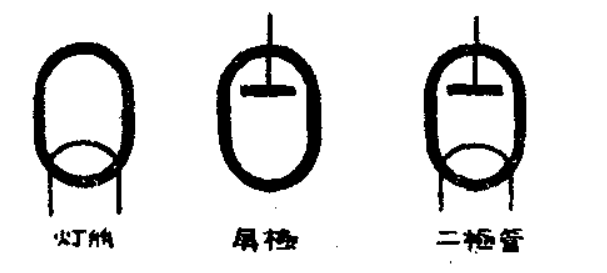
\includegraphics[width=0.5\linewidth]{diode_symbol.png}
    \caption{二极管符号}
    \label{fig:diode_symbol}
\end{figure}

\begin{figure}[H]
	\centering
	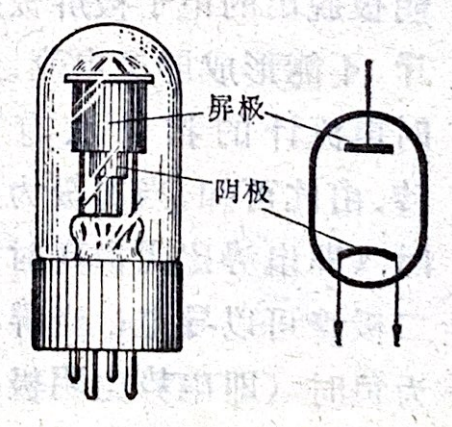
\includegraphics[width=0.6\linewidth]{diode-structure-photo.png}
	\caption{二极管电子管实物结构示意图（左：实物图；右：符号图）}
	\label{fig:diode-structure-photo}
\end{figure}

金属丝或金属管中的自由电子，像气体中的分子一样，在不停地作无规则运动。当金属受热温度升高时，电子无规则运动的动能也就跟着增加，一些动能特别大的电子，就有可能脱出金属形成所谓\textbf{热电子}。高速自由电子脱出金属的过程和液体蒸发的过程非常相似。

脱出的热电子聚集在金属表面附近的空间里，形成所谓\textbf{电子云}，如图\ref{fig:electron-cloud}所示。这时电子云里的电子仍旧在作无规则的运动。

\begin{figure}[H]
	\centering
	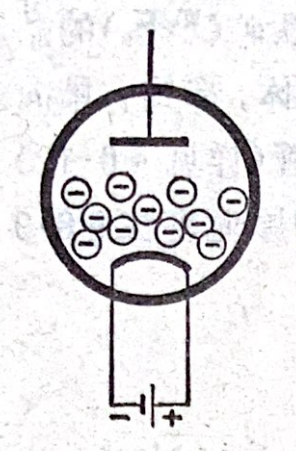
\includegraphics[width=0.6\linewidth]{electron-cloud.png}
	\caption{热电子发射与电子云示意图}
	\label{fig:electron-cloud}
\end{figure}

\section{二极管的单向导电性}

二极管工作时需要两组电源：一组为灯丝（直热式阴极）供电，称为"甲电"，电流通过灯丝产生热量使其发射电子；另一组为屏极提供工作电压，称为"乙电"。

如果把二极管电子管的屏极和阴极分别和乙电的正极和负极相接通，并在电路中串联一只电流计，这就构成一个如图\ref{fig:plate-circuit}(a)所示的屏极电路。这时，相对于阴极来说，屏极的电势较高，在两极间有电场存在。由阴极脱出的电子，在电场的作用下流向屏极，形成了电流（电流和电子流的方向相反，在电子管内电流的方向从屏极流向阴极）。这个电流叫做\textbf{屏极电流}或"屏流"。

\begin{figure}[H]
	\centering
	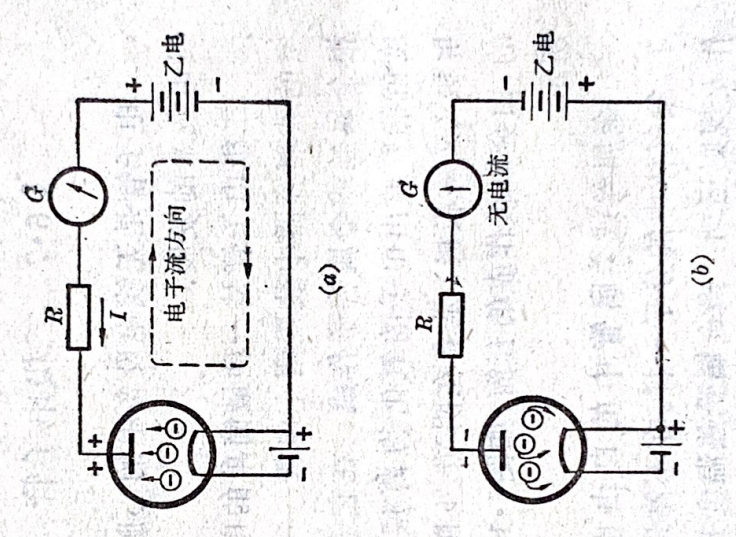
\includegraphics[width=0.8\linewidth]{diode-plate-circuit.png}
	\caption{二极管屏极电路（a）正向连接；（b）反向连接}
	\label{fig:plate-circuit}
\end{figure}

如果把乙电的正负极对调，如图\ref{fig:plate-circuit}(b)所示，那么屏极比阴极的电势较低，从阴极脱出的电子被屏极推斥，不能形成屏极电流。此时电流计的指针没有偏转。

由此可知，当屏极为正时（即电势比阴极高时），二极管可以导电；当屏极为负时（即电势比阴极低时），二极管不能导电。这种\textbf{单向导电性}（电流只能从阴极流向阳极）是真空二极管的核心特性，使其成为理想的单向导电阀。

这一特性有两大重要应用：一是在无线电接收中用于检波——当调谐电路将已调好的高频电流送到屏极时，正半周时屏极带正电，检波电路有电流通过；负半周时屏极带负电，电子流被排斥，电流不通。经过听筒的电流成为脉动直流，其振幅与输入的高频电流相同，因此能听到播音。二是用于整流——将交流电转换为直流电，这在电源供应设备中至关重要。

\begin{figure}[H]
    \centering
    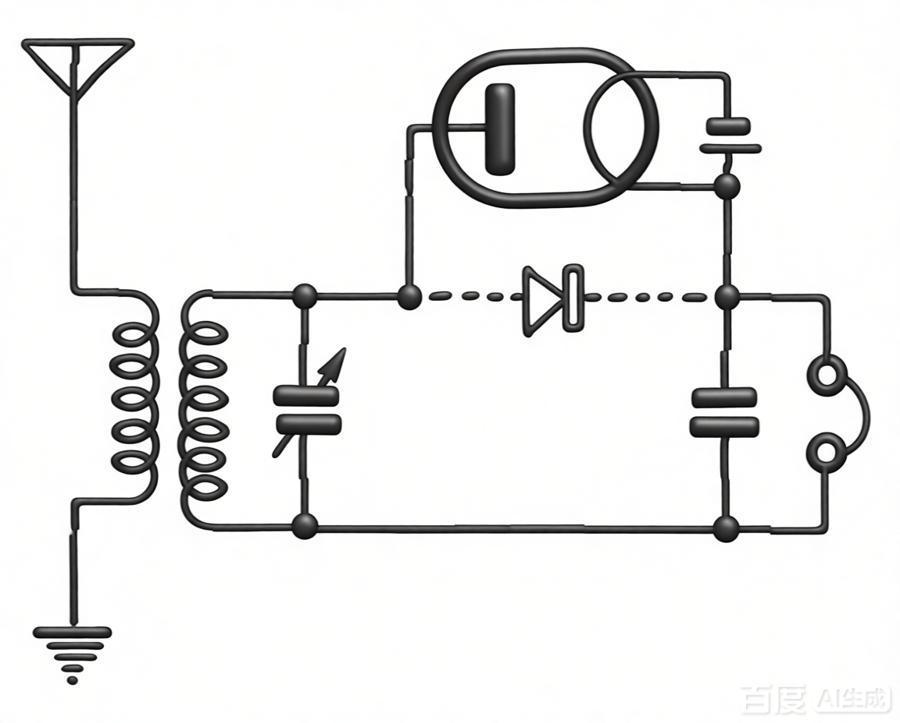
\includegraphics[width=0.8\linewidth]{diode_detector_circuit.jpg}
    \caption{二极管检波电路}
    \label{fig:diode_detector_circuit}
\end{figure}

二极管检波器的最大优势是工作稳定，不像矿石检波器那样因灵敏点接触变化而影响收音效果。但其缺点也很明显：灯丝需要消耗电能，且本身没有信号放大能力，通过听筒的仍是天线上的微弱电流，音量无法提升。

弗莱明发明的这一器件被称为"弗莱明阀"，标志着电子管时代的开端。但要实现真正实用的无线电接收，还需要能够放大微弱信号的器件——这正是真空三极管要解决的问题。

\section{各极电压与屏极电流的关系}

各极电压与屏极电流的关系如下：

当屏极电压保持不变时，改变灯丝电压会影响屏极电流：电压升高使灯丝温度上升，电子发射量增加，屏极电流随之增大；反之，降低甲电电压会使灯丝温度降低，电子发射量减少，屏极电流随之减小。但这种做法会缩短灯丝寿命，甚至导致烧毁。因此，实际应用中灯丝电压都有额定值，灯丝的电子发射能力保持恒定。

在灯丝电压固定的情况下，改变屏极电压会对屏流产生影响：当乙电电压增加时，屏极吸收电子的能力增强，屏流随之增加。但由于灯丝发射的电子数量有限，当所有电子都被屏极吸收后，再增加屏压也不会使屏流继续增大，此时的屏流称为\textbf{饱和屏流}。

当降低屏极电压时，屏流随之减少。此时并非所有电子都被吸收，未被吸收的电子会聚集在阴极附近，形成带负电的"电子雾"。这些积累的电子被称为\textbf{空间电荷}，它们会产生排斥电场，限制阴极继续发射电子。即使阴极持续发射新电子，空间电荷区域也会迅速达到动态平衡，新发射的电子会补充被吸收的电子位置。

"电子雾"的分布与屏极电压和阴极电压都有关系。在屏极电压固定的情况下，若降低阴极电压，电子发射量减少，屏极能够吸收全部电子，此时不存在空间电荷；若提高阴极电压，电子发射量增加，空间电荷会显著增多。但由于空间电荷会排斥新发射的电子，其总量不会无限增大，而是达到动态平衡。

空间电荷会阻碍屏极吸收电子。为了克服这种阻碍，需要提高屏极电压以增强对电子的吸引力，这会导致功率消耗增加。因此，空间电荷对电子管的工作是有害的。

\chapter{二极管整流电路}

二极管的单向导电性使其成为理想的整流元件。所谓\textbf{整流}，就是将交流电转换为直流电的过程。在电子设备中，电源通常来自交流电网，而电子管等器件需要稳定的直流电源才能工作，因此整流电路是电子设备中不可或缺的组成部分。

\section{半波整流电路}

在无线电电子仪器中常需要电流不大的直流电源，通过电子管整流器就可把交流电变成直流电。图\ref{fig:half-wave-rectifier}是常见的半波整流电路。当变压器T的初级线圈与交流电源接通后，由于变压器的作用，在次级线圈中产生了感应电压。

\begin{figure}[H]
	\centering
	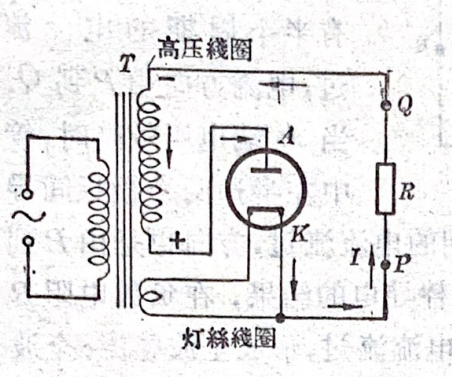
\includegraphics[width=0.7\linewidth]{half-wave-rectifier.png}
	\caption{半波整流电路}
	\label{fig:half-wave-rectifier}
\end{figure}

当A端为正时，即二极管屏极电压高于阴极时，二极管导电，整流电流就沿图中箭头方向流经负载电阻R。当交流电压变化到K端为正时，屏极电压低于阴极电压，二极管不导电（可见交流电只有半个周期被利用）。再过半个周期，交流电压又变化到A端为正，又有方向与前一次一样的电流流过R，这样负载电阻R上就只有单向的电流流过，形成了半波整流电流。

电压曲线如图\ref{fig:half-wave-waveform}(a)所示，整流后的波形如图\ref{fig:half-wave-waveform}(b)所示。由此可见，R两端的电势总是P端高Q端低，但PQ之间的电压却仍然是变动着的，而且每隔半周，电压就有一次为零，输出的电压是不稳定的。半波整流电路结构简单，但效率较低，只利用了交流电的一半周期。

\begin{figure}[H]
	\centering
	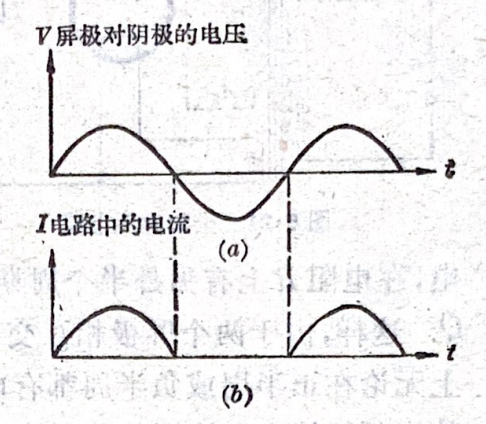
\includegraphics[width=0.8\linewidth]{half-wave-waveform.png}
	\caption{半波整流波形图（a）输入交流电压；（b）输出脉动直流电压}
	\label{fig:half-wave-waveform}
\end{figure}

\section{全波整流电路}

要获得比较稳定的直流电源，必须使用全波整流器。全波整流是由双二极管的电路来完成的，如图\ref{fig:full-wave-rectifier}所示。实际上，它相当于两个半波整流器组合而成。

\begin{figure}[H]
	\centering
	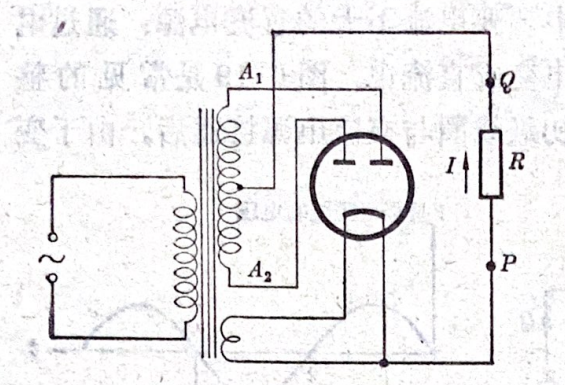
\includegraphics[width=0.8\linewidth]{full-wave-rectifier.png}
	\caption{全波整流电路（双二极管结构）}
	\label{fig:full-wave-rectifier}
\end{figure}

当变压器次级线圈的$A_1$端电压较高时，管中右半边的两个极板间导电，在负载电阻$R$上有半个周期的电流流过，电流方向由$P$到$Q$。当$A_2$端电压较高时，管中左半边两个极板间导电，在电阻$R$上有另外半个周期的电流流过，方向也是由$P$到$Q$。

这样，由于两个屏极相互交替导电的结果，在负载电阻$R$上无论在正半周或负半周都有电流流过，形成全波整流。全波整流不仅输出电流平均值比半波整流大，并且波形也比半波整流稳定得多。

\begin{figure}[H]
	\centering
	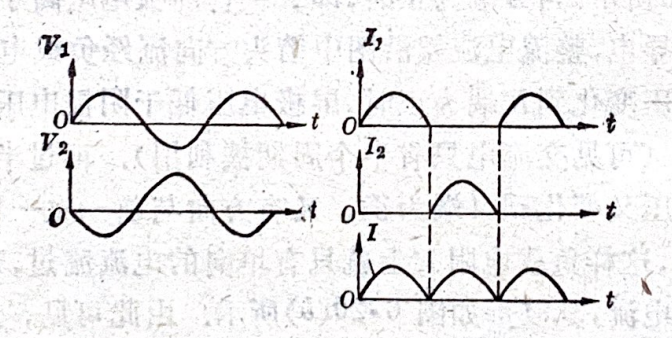
\includegraphics[width=0.8\linewidth]{full-wave-waveform.png}
	\caption{全波整流波形图（电流强度随时间变化，但方向始终不变）}
	\label{fig:full-wave-waveform}
\end{figure}

图\ref{fig:full-wave-waveform}所示的图线，表示电流强度随时改变，但方向始终不变的电流，这种电流叫做\textbf{脉动电流}。

\part{真空三极管与电子学时代}

\chapter{真空三极管的发明}

这一关键突破来自美国发明家德·福雷斯特。1906年，他在二极管的阴极和阳极之间引入了第三个电极——用金属丝制成的栅网状或螺管形结构，将阴极包围起来，称为\textbf{控制栅极}。这一新型器件被称为\textbf{真空三极管}。

\section{栅极的控制作用}

在屏极、阴极间添加了栅极后就构成了三极电子管。栅极是套在阴极的外面，用金属导线绕在支柱上的圆柱形或扁盒形的稀疏网，它离阴极很近，如图\ref{fig:triode-grid-structure}所示。栅极可以控制电子管的电子流，使电子管能作更多的工作。

\begin{figure}[H]
	\centering
	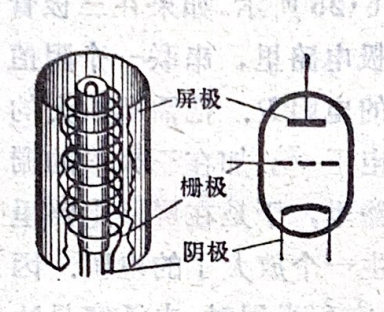
\includegraphics[width=0.6\linewidth]{triode-grid-structure.png}
	\caption{真空三极管栅极结构示意图}
	\label{fig:triode-grid-structure}
\end{figure}

栅极的加入是一项革命性的创新。它位于阴极附近，处于电子从阴极飞向阳极的路径上。由于栅极与阴极距离很近，即使在栅极上施加很小的电压变化，也能显著改变阴极附近的电场分布，从而精确控制电子管内的电子流。这类似于通过微调水龙头阀门来控制水流大小——加在栅极上的微弱信号可以在阳极电路中产生波形相同但幅度显著放大的信号，\textbf{信号放大功能}由此实现。

如图\ref{fig:grid-control-field}所示，用丙电池使栅极带上正电，那么栅极和屏极会产生一个相当强大的合成电场，使从阴极脱出的电子所受的电场力加大，也就是电子的运动速度加快。同时使通过栅极飞向屏极的电子数目大为增多，因而屏极电流增大。其中也有一小部分电子到达栅极时，从栅极电路流回阴极，产生了栅极电流。

\begin{figure}[H]
	\centering
	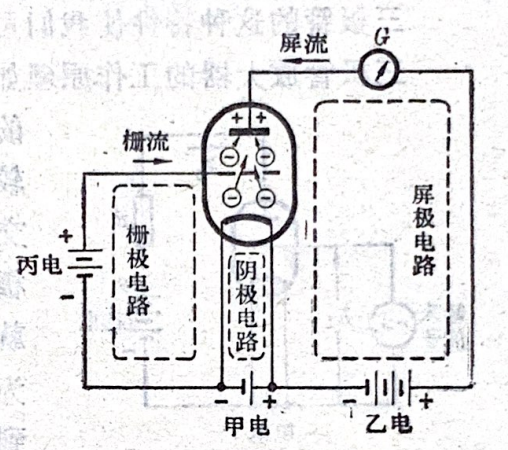
\includegraphics[width=0.7\linewidth]{grid-control-field.png}
	\caption{栅极控制电场示意图（左：正栅压；右：负栅压）}
	\label{fig:grid-control-field}
\end{figure}

如果把丙电池的正负极倒接过来，使栅极带上负电，那么它就会削弱屏极对电子的吸引力，也就是减小屏极电流。同时由于栅极电压比阴极电压低，因而它推斥电子，不会产生栅极电流。可见改变栅极的电压（栅极和阴极间的电势差，在无线电技术中常称为栅极电压。因为一般常把阴极接地，它的电势为零），就能控制屏极电流的变化。

三极管工作时除了甲电和乙电，还需要在栅极与阴极之间接入第三组电源——通称"丙电"，形成"栅极电路"。当丙电正极接栅极使栅极带正电时，它与带正电的屏极产生合成电场，增强屏极对电子的吸引力，使屏流增加；同时会有一小部分电子被栅极吸收，形成"栅极电流"。若将丙电反接使栅极带负电，其电场与屏极相反，削弱屏极吸引力，屏流减少，且栅极排斥电子不会产生栅极电流。当栅极负电压足够大时，排斥力超过屏极吸引力，电子无法到达屏极，屏流完全截止。

栅极正电压过高时，全部发射电子被栅极和屏极吸收，再增加栅压屏流也不再增加，此时达到"屏流饱和点"；栅极负电压过高时，全部电子被拒斥，屏流被切断，此时的丙电电压称为"切断负压"。

如果将交流电压输入栅极，当它的最大值在正半周不超过屏流饱和点、负半周不低于屏流切断点时，这种正负变化就能使屏极电流产生相应变动，如图\ref{fig:grid_voltage_waveform}所示。

\begin{figure}[htbp]
    \centering
    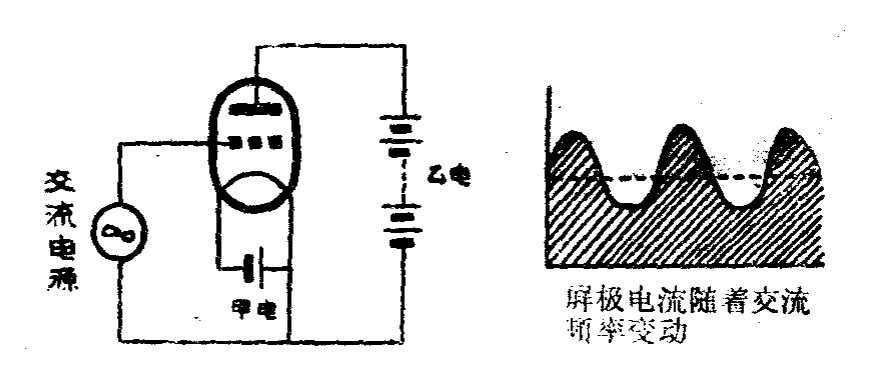
\includegraphics[width=0.7\linewidth]{grid_voltage_waveform.png}
    \caption{栅极电压与屏极电流波形}
    \label{fig:grid_voltage_waveform}
\end{figure}

我们知道，如果改变屏极电压（屏极和阴极间的电势差），也能引起屏极电流的变化，但栅极离开阴极比屏极离开阴极近得多，因此栅极电压的变化所引起的屏极电流的变化，要比屏极电压的变化所能引起的大得多。总的来说，\textbf{栅极电压作微小的变化，就能引起屏极电流作相当大的变化}。

三极管的这种特性使我们可能利用它来作为放大器。因此，栅极的作用可以理解为：栅极上较小的电压变动，便能使屏流发生很大变化，所以栅极有时也被称为"控制栅"。

当栅极用于控制屏流时，通常会施加一个较小的负电压，这能使电子管工作在良好的特性区域，并且避免栅极吸收电子而消耗功率。这个电压称为"栅偏压"（或丙电压）。

\section{三极管的基本功能与影响}

由于三极管栅极的控制作用，这类电子管能够实现检波功能，对高频和低频信号进行放大，还能产生振荡。这些基本功能具有多样化且突出的特性，使得微弱的无线电信号可以被多级放大以驱动扬声器，稳定的高频振荡电路得以实现为无线电台载波发射奠定基础，长途电话信号放大成为可能，电视和雷达等新技术的研究也随之展开。

从收音机的普及和广播事业的兴起，到早期电子计算机的发展和现代电子工业的建立，真空三极管都起到了奠基性的作用。德·福雷斯特的这一发明开创了电子学的新时代。

\section{放大器的分类}

放大器的种类很多，按任务分有电压放大器和功率放大器等，按频率范围分有高频放大器和低频放大器（即音频放大器）等，在无线电发送机和接收机里或电子仪器里，放大器被广泛地应用着。

\chapter{三极管的基本电路}

所有三极管电路都可以分为三个基本电路：阴极电路、栅极电路（又叫输入电路）和屏极电路（又叫输出电路）（图\ref{fig:triode_circuit}）。三个电路的公共点0叫做电路的"零点"。

\begin{figure}[htbp]
    \centering
    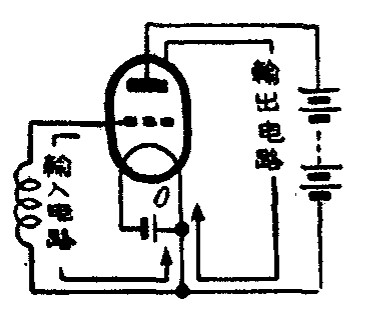
\includegraphics[width=0.7\linewidth]{triode_circuit.jpg}
    \caption{栅极电路和屏极电路}
    \label{fig:triode_circuit}
\end{figure}

因为屏极通常接正电压，所以有时叫它"阳极"；相对于阳极而言，发射电子的阴极也叫做"阴极"。

三极管是无线电技术里最基本的电子管，它的各种作用和实际应用，我们将在下面和以后逐一讲到。

\chapter{三极管的检波作用}

三极管也能进行检波作用，其检波作用比二极管优良得多。三极管检波器有两种——屏极检波和栅极检波。

\section{屏极检波}

屏极检波是依靠电子管的特性来实现的。利用三极管的屏极电路进行检波工作的，叫做屏极检波法。电路如图\ref{fig:plate_detector}所示。在栅极接上一个丙电（栅偏压电源），使它带有相当高的负电压，使屏极电流刚好截止。当已调幅高频电压加到栅极上时，只有正半周能使电子管产生屏极电流，从而完成检波任务。

\begin{figure}[htbp]
    \centering
    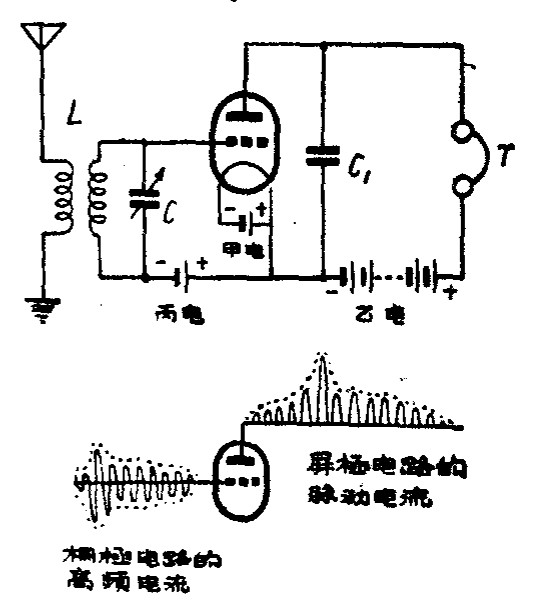
\includegraphics[width=0.7\linewidth]{plate_detector.jpg}
    \caption{屏极检波电路}
    \label{fig:plate_detector}
\end{figure}

调谐电路与栅偏压电源（丙电）串联。当输入信号处于正半周时，信号电压抵消了一部分栅极负偏压，产生屏极电流，其大小随输入信号幅度变化。当信号进入负半周时，信号电压与栅极负偏压叠加，使栅极负电压增大，从而切断屏极电流。将耳机串联在屏极电路中，正半周时有半周屏流通过，负半周时无电流通过。这样耳机中就产生了脉动电流，其幅度随输入信号变化，驱动耳机振膜振动发声。

屏极检波是在屏极电流上取得半周电流来完成检波工作的。这半周电流的变化与输入信号的音频变化相同，但幅度远大于输入信号，因此耳机发声较为响亮。检波后残余的高频电流通过与耳机并联的"旁路电容器"（$C_1$）滤除，使耳机中只流过音频电流。

然而，屏极检波在现代收音机中应用较少，主要原因如下：

\begin{enumerate}[leftmargin=1cm]
    \item \textbf{效率较低}：屏极检波需要在栅极上施加一个较大的负偏压（通常由丙电提供），这部分偏压电源会持续消耗电能，导致整体电路效率下降。相比之下，栅极检波可以利用信号本身或自给偏压方式获得偏置，无需额外电源。
    
    \item \textbf{失真较大}：屏极检波工作在电子管的截止区附近，当信号幅度变化时，工作点会在非线性区域移动，容易产生较大的非线性失真，影响音质。而栅极检波工作在更接近线性的区域，失真较小。
    
    \item \textbf{灵敏度受限}：由于栅极负偏压的存在，需要较大的输入信号才能使电子管导通产生屏极电流，因此对微弱信号的响应能力较弱，灵敏度低于栅极检波和二极管检波。
    
    \item \textbf{电路复杂}：需要额外的丙电（栅偏压电源），增加了电路的复杂性和成本。在便携式收音机中，额外的电源意味着更大的体积和更高的功耗，这在实际应用中是不利的。
    
    \item \textbf{技术发展淘汰}：随着电子技术的进步，更高效、更稳定的检波方式不断涌现。栅极检波以其高灵敏度和低失真成为电子管收音机的主流方案，而二极管检波则以其简单可靠的特点广泛应用于各种接收机中。
\end{enumerate}

综上所述，尽管屏极检波能提供较大的输出功率，但由于上述缺点，它已逐渐被更先进的检波方式所取代。

\section{栅极检波}

利用三极管的栅极电路进行检波工作的方法，叫做栅极检波法。在栅极电路中，栅极不接入负电压，调谐电路与栅极之间连接一个"栅极电容器"（$C_1$）。输入信号的高频电流经过它到达栅极；在正半周时，栅极带正电吸收电子，但电子不能通过$C_1$完成回路，导致栅极上积存大量电子，阻碍屏极电流。因此需要在栅极和阴极之间接入一个电阻（$R$），使一部分电子通过它漏泄回阴极，这个电阻称为"栅漏电阻"。

正半周时$R$上有电流通过，负半周时栅极带负电排斥电子，$R$上没有电流。于是栅漏电阻上产生的电压降就是一个与广播信号相似的脉动电压，残余高频成分仍可从$C_1$通过。

栅极电路相当于起着二极管检波的作用（此时的栅极相当于二极管检波时的阳极），结果在栅极上形成了高频电压和音频脉动电压的叠加。

\begin{figure}[htbp]
    \centering
    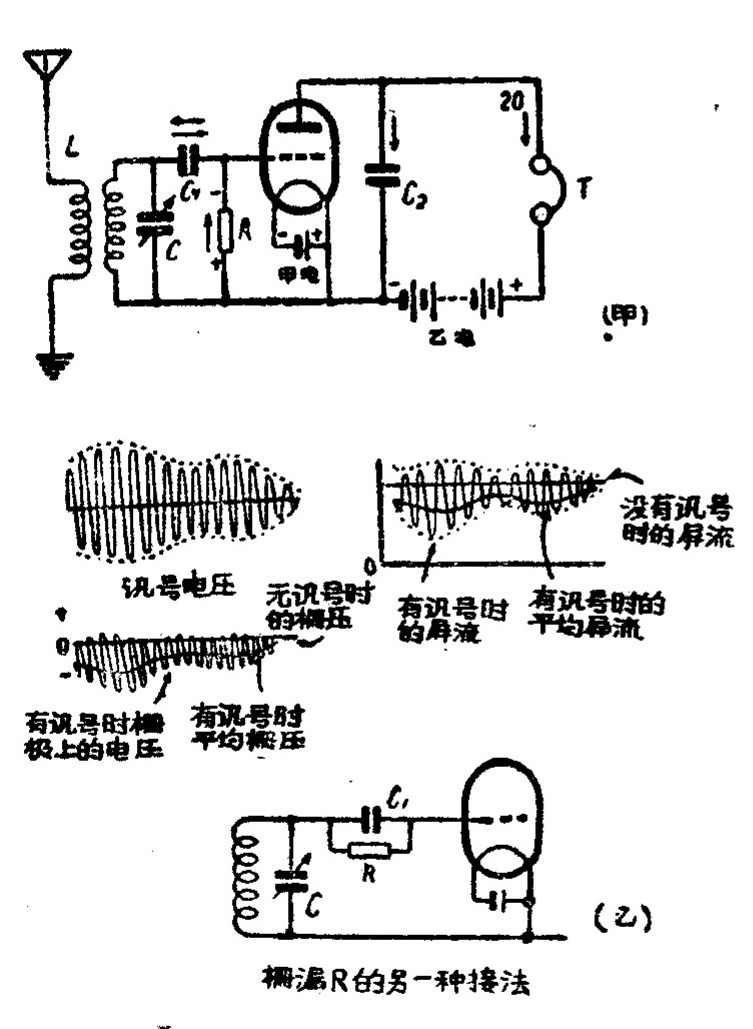
\includegraphics[width=0.8\linewidth]{grid_detector.jpg}
    \caption{栅极检波电路}
    \label{fig:grid_detector}
\end{figure}

屏极电路中，屏极电流受到栅极控制。当栅极起到二极管检波作用时，屏极电路中也会发生栅极上所有高频和音频成分的变化。高频电流从旁路电容器（$C_2$）流过后，耳机里流过的就是音频电流了。音频电流的变化与输入信号相同，但幅度要大得多。

栅极检波就是先在栅极电路检波，再在屏极电路放大。此法输出电压虽不很大，但相当灵敏，是简单电子管收音机中最常采用的电路。

栅漏电阻（$R$）有时也可与栅极电容器（$C_1$）并联，接法如图\ref{fig:grid_detector}所示，效果与图甲的接法相同。

栅极检波与其他的检波方式相比较，有较高的灵敏度，但工作时有栅极电流产生，会影响到调谐回路的质量，从而使选择性变坏，但在一般简单的收音机里，对于灵敏度的要求比其他指标更为重要，所以栅极检波仍被广泛地采用。

\chapter{电子管收音机与多极管}

\section{电子管收音机的优势}

采用电子管作为检波器后，收音机的灵敏度和选择性显著提升，性能远超矿石收音机。

尽管电子管收音机需要电源供电，但单管收音机的功耗较低，不会给普通用户带来显著的经济负担，因此这并非其主要缺点。

\section{多极管}

三极管是基本的电子管，用它几乎可以说明许多无线电电路的工作原理。虽然现在一般电路中大多采用效率更优的多极电子管，但它们都是在三极管的基础上改进而来，电路原理大同小异。

\subsection{四极管}

在屏极和栅极之间加入一个稀疏的网状电极，就构成了四极管。这个电极的作用是将屏极和栅极隔离开来，称为"帘栅"或"障栅"（图\ref{fig:tetrode_structure}）。在电路中，通常将它接入一个低于或相当于屏极的正电压，因此它也能吸收电子产生"帘栅电流"。不过由于它是稀疏的栅网，吸收电子的数量有限，大部分电子仍被屏极吸收。

帘栅在屏极前方产生一个强大的电场，对空间电荷有直接影响，从而减弱了屏极对空间电荷的作用，使得屏极电压的变化对屏极电流的影响减小。结果是控制栅对屏极电流的影响相对增大，即控制栅的效率得到了提高。

\begin{figure}[htbp]
    \centering
    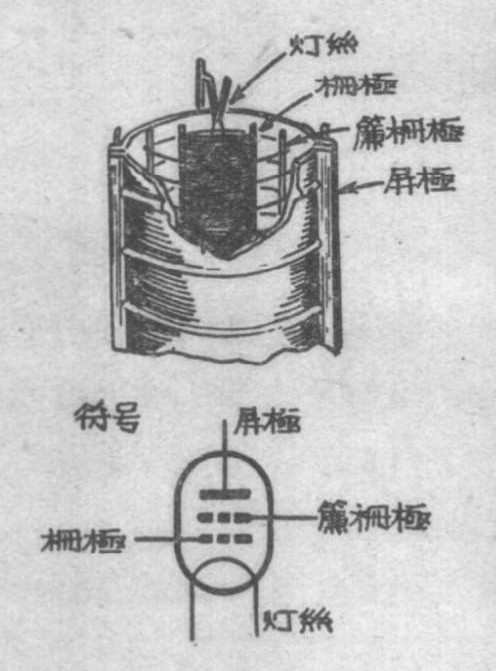
\includegraphics[width=0.7\linewidth]{tetrode_structure.jpg}
    \caption{四极管结构}
    \label{fig:tetrode_structure}
\end{figure}

\begin{figure}[htbp]
    \centering
    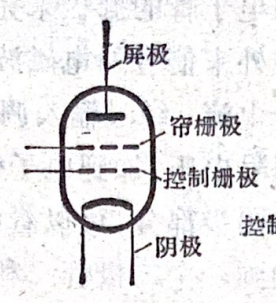
\includegraphics[width=0.5\linewidth]{tetrode_symbol.png}
    \caption{四极管符号}
    \label{fig:tetrode_symbol}
\end{figure}

其次，三极管中各个电极之间都可看作是微小的电容器，虽然电容量很小，但在高频工作时仍会产生影响，尤其是屏极和栅极之间的电容影响最大（图\ref{fig:interelectrode_capacitance}）。加入帘栅后，将屏极和栅极分隔开，形成两个串联的电容器，从而将总电容量降到很低，因此四极管在高频工作时性能远优于三极管。

\begin{figure}[htbp]
    \centering
    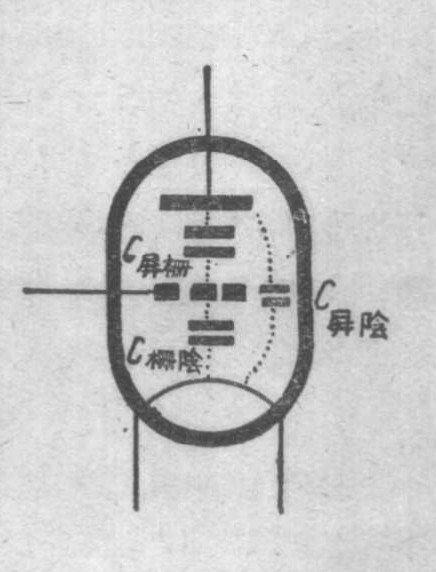
\includegraphics[width=0.7\linewidth]{interelectrode_capacitance.jpg}
    \caption{极间电容示意图}
    \label{fig:interelectrode_capacitance}
\end{figure}

然而四极管也有显著缺点：由于帘栅的存在使电子流加速，当高速电子冲击屏极时，会撞击出屏极的电子，形成二次电子发射。这些二次电子若能立即被屏极吸收回去影响不大，但电子管工作时，屏极电压有时会低于帘栅电压，此时二次电子会被帘栅吸收，导致帘栅电流迅速上升，同时到达屏极的电子减少，屏极电流下降，使电子管工作不稳定。

这个缺点使得四极管在收音机中应用较少。

\subsection{五极管}

为了克服四极管的缺点，设计者在屏极和帘栅之间再加入一个新的栅极，称为"抑制栅"或"遏止栅"（图\ref{fig:pentode_structure}）。它通常与阴极相连，电位为零，成为屏极和帘栅的静电隔离层。当发生二次电子发射时，抑制栅能将电子排斥回屏极，从而抑制帘栅吸收二次电子，大幅提高电子管的性能。

\begin{figure}[htbp]
    \centering
    %\includegraphics[width=0.7\linewidth]{pentode_structure.jpg}
    \caption{五极管结构}
    \label{fig:pentode_structure}
\end{figure}

五极管适用于各种放大工作，是目前最流行的电子管之一。

五极管的符号如图\ref{fig:pentode_symbol}所示，其结构特点是：最靠近阴极的栅极是控制栅（又称第一栅）；其次是帘栅（又称第二栅）；靠近屏极的是抑制栅（又称第三栅）。

\begin{figure}[htbp]
    \centering
    
\includegraphics[width=0.5\linewidth]{pentode_symbol.jpg}
    \caption{五极管符号}
    \label{fig:pentode_symbol}
\end{figure}

\subsection{集射式四极管}

另一种能够克服二次电子发射影响的电子管是"集射式"四极管。普通阴极发射电子时是向四周扩散的；集射式电子管则在帘栅和屏极之间相对放置一对金属板，称为"电子束形成极"。它与阴极连接处于零电位，两边各留出一个"缺口"。电子从阴极发射出来后被这两块金属板排斥，只能集中从"缺口"冲出，形成一束强烈的电子流。

另一方面，栅极和帘栅的圈数相同且每圈彼此相对，电子束冲出时由于栅极带负电而被分成一排排，帘栅恰好处于每排电子束的"间隙"中，吸收电子的机会大为减少。同时，因电子集中在若干束内，在屏极前密度很大，能够将屏极射出的二次电子赶回屏极，避免被帘栅吸收。

集射式四极管的构造和工作情形如图\ref{fig:beam_tetrode}所示。电子束形成极在这里只作为辅助电极，因此这类电子管仍属于四极管。

\begin{figure}[htbp]
    \centering
    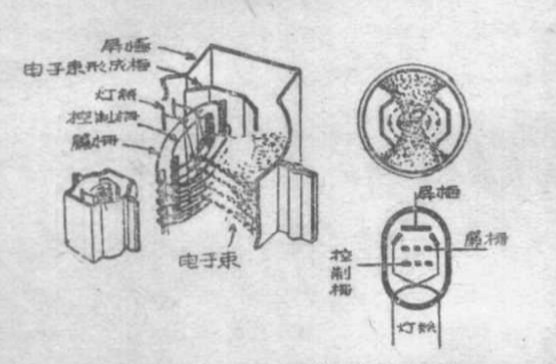
\includegraphics[width=0.8\linewidth]{beam_tetrode.jpg}
    \caption{集射式四极管的构造}
    \label{fig:beam_tetrode}
\end{figure}

在许多情况下，集射式四极管可以代替强力五极管，且性能更优。这类电子管在我国也有称为"束流管"、"集流管"或"电子注管"等名称。

\subsection{复合管}

有时为了使用方便和节省空间，可以将两个（或几个）电子管合装在一个真空玻璃泡内，称为"复合管"。大多数复合管还可以共用一个公共阴极，但管内每个"电极组"的作用仍然各自独立，不会相互影响。在后续的多管收音机中，我们也会使用到复合管。

\section{常用电子管的型式}

电子管的制造有多种不同的结构形式，在安装技术中需要充分了解它们的安装方法。下面列举一些常用的和国产的电子管型式。

\subsection{玻璃式}

这类电子管的外壳由玻璃制成，固定在一个胶木的"管腰"上。各电极通过导线从管内引出，焊接在管腰下方的"管脚"（插脚）内，以便插入"管座"（图\ref{fig:glass_tube}）。由于电极数目不同，插脚数目也不同，通常分为4脚式、5脚式、6脚式和7脚式四种。有时控制栅从管子顶部引出，连接在金属"管顶"上。这种型式在老式收音机中还能见到，但近来已很少使用。

\begin{figure}[htbp]
    \centering
    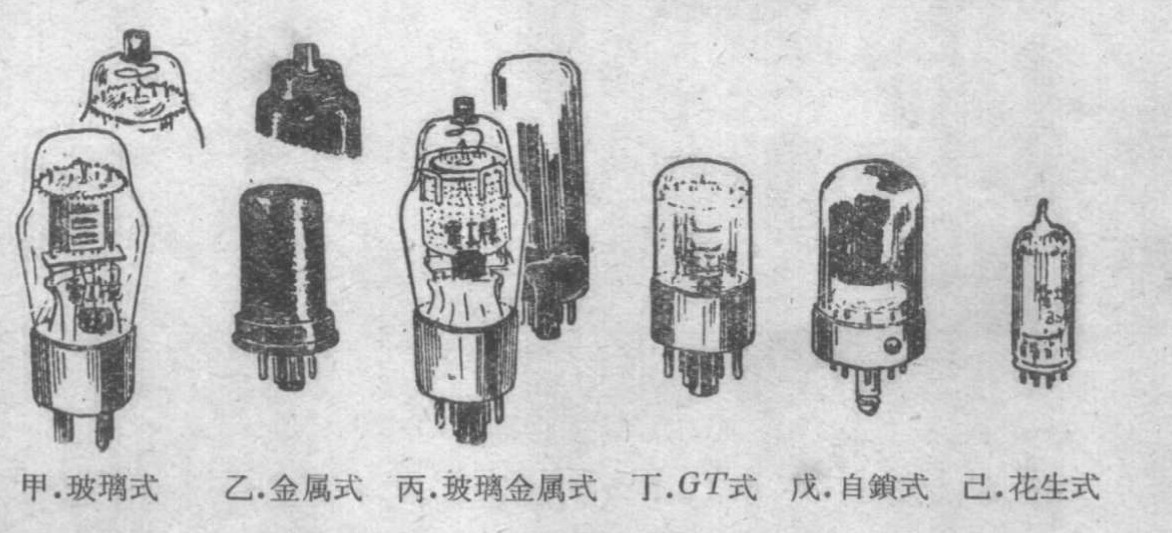
\includegraphics[width=0.7\linewidth]{glass_tube.jpg}
    \caption{玻璃式电子管（图甲）}
    \label{fig:glass_tube}
\end{figure}

\subsection{金属式}

金属式电子管在制造上更为先进。外壳用铁皮制成，因此无法窥见内部结构（图\ref{fig:metal_tube}）。这种结构能隔离电子管与外界的不必要感应，散热更容易，体积也更小，内部接线可以缩短。不过内部电极的支持座和抽气口仍用玻璃制造，长期使用中由于冷热交替，玻璃与金属的结合处可能会产生漏气现象，导致电子管效率降低或失效。

\begin{figure}[htbp]
    \centering
    %\includegraphics[width=0.7\linewidth]{metal_tube.jpg}
    \caption{金属式电子管（图乙）}
    \label{fig:metal_tube}
\end{figure}

金属式电子管的另一个特点是：不论内部电极多少，插脚一律采用"八脚式"，其中有一个"对正键"，便于插入管座时不会插错。

但使用干电池作为甲电电源的电子管，几乎没有金属式的。

\subsection{玻璃金属式}

将金属式电子管的外壳改为玻璃材质，就成为玻璃金属式电子管（图\ref{fig:glass_metal_tube}），通常称为"G"式管。其内部电极构造和插脚排列与金属式完全相同，只需在金属管型号后加一个"G"字。例如：金属管6F6改为这种型式，就叫做6F6G。苏联的这类电子管则在型号后加一个"C"字，例如金属管6Ф6的玻璃金属式就是6Ф6C。

\begin{figure}[htbp]
    \centering
    %\includegraphics[width=0.7\linewidth]{glass_metal_tube.jpg}
    \caption{玻璃金属式电子管（图丙）}
    \label{fig:glass_metal_tube}
\end{figure}

\subsection{GT式}

玻璃金属式电子管体积与玻璃式一样较为笨重，后来制造商将其缩小到与金属式差不多的尺寸，称为"GT"式（图\ref{fig:gt_tube}），型号后加GT两个字母。例如：6F6G制成这种型式，就叫做6F6GT（苏联同类型管子后加-M字，例如6Ф6M、6Ф5M等）。

在我国有些地方，这种型式也被称为"小鸡式"。

\begin{figure}[htbp]
    \centering
    %\includegraphics[width=0.7\linewidth]{gt_tube.jpg}
    \caption{GT式电子管（图丁）}
    \label{fig:gt_tube}
\end{figure}

\subsection{自锁式}

自锁式电子管的玻璃泡与GT式相似，但管腰较矮，由金属制成，上面有一个圆点突出作为插入管座的标记。各电极的支柱直接伸出作为插脚，也是八脚式（但与上述八脚式不同）（图\ref{fig:self_locking_tube}）。对正键的末端有一圈小槽，插入管座后会被管座上特制的弹簧套住，不易跳出，因此称为自锁式（苏联这类电子管型号后带一个"Л"字）。

\begin{figure}[htbp]
    \centering
    %\includegraphics[width=0.7\linewidth]{self_locking_tube.jpg}
    \caption{自锁式电子管（图戊）}
    \label{fig:self_locking_tube}
\end{figure}

\subsection{花生式}

在常用电子管中，花生式的体积较小，整体由玻璃制成，尺寸约为一颗花生大小（图\ref{fig:peanut_tube}），插脚一律为7只。苏联同类电子管称为"姆指管"，型号后带一个"П"字。

\begin{figure}[htbp]
    \centering
    %\includegraphics[width=0.5\linewidth]{peanut_tube.jpg}
    \caption{花生式电子管（图己）}
    \label{fig:peanut_tube}
\end{figure}

\section{电子管的分类和电子管特性表}

电子管应用非常广泛，且有各种型式，种类繁多。通常按型式、构造、用途等进行分类（从前还有以其他方式分类的）。

每一种型号的电子管都有其独特特性，为了参考方便，通常按一定方法（如字母顺序、数字）排列，将它们的性能列成表格，称为"电子管特性表"。在特性表上，可以查找每一种电子管的各种数据、性能以及管座接线图等，非常方便。

不同国家的电子管命名体系有所不同。有些国家的电子管型号命名较为复杂，存在一定的重复。而苏联的电子管型号按照统一的全苏标准制定，每个字母和数字都表示特定意义，使用起来较为方便。

\subsection{苏联电子管命名规则}

苏联电子管型号通常由四部分组成：

\begin{enumerate}
    \item \textbf{第一部分（数字）}：表示灯丝电压（单位：伏特）
    \item \textbf{第二部分（字母）}：表示电子管型式（程式）
    \item \textbf{第三部分（数字）}：表示厂家特定的序号
    \item \textbf{第四部分（字母）}：表示构造型式
\end{enumerate}

其中第二个字母的含义如下：
\begin{description}
    \item[Д] 二极管
    \item[П] 输出五极管及集射管
    \item[Х] 双三极管
    \item[Г] 附二极管的三极管
    \item[С] 三极管
    \item[Б] 附二极管的五极管
    \item[К] 遥截止管
    \item[Н] 双三极管
    \item[Ж] 锐截止五极管
    \item[Ф] 三极-五极管
    \item[А] 双控制栅变频管
    \item[Л] 整流管
\end{description}

第四个字母表示构造型式：
\begin{description}
    \item[М] 金属玻璃式管（即GT式）
    \item[С] 玻璃管
    \item[Л] 自锁式
    \item[П] 姆指管（花生式）
    \item[Б] 超小型管（直径10公厘）
    \item[А] 特小型管（直径6公厘）
\end{description}

金属管则无第四个字母。

\subsection{中国电子管命名规则}

我国电子管命名体系参考了苏联标准并结合实际情况制定，型号通常由三到四部分组成：

\begin{enumerate}
    \item \textbf{第一部分（数字）}：表示灯丝电压（单位：伏特）
    \item \textbf{第二部分（字母）}：表示电子管类型
    \item \textbf{第三部分（数字）}：表示产品序号
    \item \textbf{第四部分（字母，可选）}：表示结构形式或改进型号
\end{enumerate}

常见的第二个字母含义：
\begin{description}
    \item[D] 二极管（如6D1、6D2）
    \item[C] 三极管（如6C1、6C2）
    \item[N] 双三极管（如6N1、6N2）
    \item[P] 五极管（如6P1、6P6P）
    \item[Z] 整流管（如6Z4、5Z3P）
    \item[F] 锐截止五极管（如6F1、6F2）
    \item[S] 束射四极管（如6S6）
\end{description}

常见型号示例：
\begin{description}
    \item[6P1] 6V灯丝，五极管，序号1
    \item[6N1] 6V灯丝，双三极管，序号1
    \item[6Z4] 6V灯丝，整流管，序号4
    \item[6P6P] 6V灯丝，五极管，序号6，玻璃壳
\end{description}

\subsection{美国电子管命名规则}

美国电子管命名体系较为多样化，不同厂家有各自的命名方式，但也存在一些通用规律：

\subsubsection{通用电子管型号（RCA标准）}
\begin{enumerate}
    \item \textbf{前缀字母（可选）}：表示特殊用途或等级（如JAN-表示军品级）
    \item \textbf{数字部分}：通常包含多位数字
    \item \textbf{后缀字母}：表示改进型号或封装形式
\end{enumerate}

常见美国电子管型号示例：
\begin{description}
    \item[12AX7] 双三极管，广泛用于音频放大（ECC83欧洲等效型号）
    \item[6V6] 束射四极管，功率放大管（6P6P中国等效型号）
    \item[6L6] 束射四极管，大功率放大管
    \item[5Y3] 整流管
    \item[JAN-5670] 军品级双三极管
\end{description}

\subsubsection{美国电子管型号特点}
- 数字通常表示灯丝电压和其他参数的组合
- 型号命名相对自由，不同厂家可能有不同命名
- 部分型号直接标注用途（如"6SN7GT"中的GT表示玻璃金属式）

\subsection{欧洲电子管命名规则}

欧洲各国电子管命名体系各有特点，以下是主要国家的命名方式：

\subsubsection{德国电子管命名规则}
德国电子管型号通常遵循以下格式：
\begin{enumerate}
    \item \textbf{字母前缀}：表示电子管类型
    \item \textbf{数字部分}：表示规格参数
    \item \textbf{字母后缀}：表示改进型号
\end{enumerate}

常见德国电子管型号示例：
\begin{description}
    \item[EL34] 五极管功率放大管（6CA7美国等效型号）
    \item[ECC83] 双三极管（12AX7美国等效型号）
    \item[EBC33] 三极-五极管变频管
    \item[EZ81] 全波整流管（6CA4美国等效型号）
\end{description}

\subsubsection{欧洲通用命名体系}
欧洲电子管型号字母含义：
\begin{description}
    \item[E] 表示接收管（Empfänger）
    \item[A/B/C/D] 表示结构类型（A=直热式，B=旁热式等）
    \item[数字] 表示序号
    \item[额外字母] 表示特殊特性
\end{description}

\subsubsection{英国电子管命名规则}
英国电子管型号通常以字母开头，如：
\begin{description}
    \item[CV系列] 军用电真空器件标准（如CV4004=12AX7）
    \item[KT系列] 束射四极管（如KT88、KT66）
\end{description}

\subsection{各国电子管型号对照}

为了方便读者查阅不同国家生产的等效电子管，下面列出常见型号的对照表：

\begin{table}[htbp]
    \centering
    \caption{各国电子管型号对照}
    \label{tab:tube_cross_reference}
    \begin{tabular}{|c|c|c|c|}
        \hline
        美国型号 & 欧洲型号 & 中国型号 & 类型 \\
        \hline
        12AX7 & ECC83 & - & 双三极管 \\
        \hline
        12AU7 & ECC82 & - & 双三极管 \\
        \hline
        12AT7 & ECC81 & - & 双三极管 \\
        \hline
        6V6 & - & 6P6P & 束射四极管 \\
        \hline
        6L6 & - & - & 束射四极管 \\
        \hline
        6CA7 & EL34 & - & 功率五极管 \\
        \hline
        6CA4 & EZ81 & - & 整流管 \\
        \hline
        5Y3 & - & - & 整流管 \\
        \hline
        5Z3 & - & 5Z3P & 整流管 \\
        \hline
        6SN7 & ECC32 & - & 双三极管 \\
        \hline
        6SL7 & ECC35 & - & 双三极管 \\
        \hline
        - & - & 6P1 & 五极管 \\
        \hline
        - & - & 6N1 & 双三极管 \\
        \hline
        - & - & 6Z4 & 整流管 \\
        \hline
        CV4004 & ECC83 & - & 双三极管（英国军用） \\
        \hline
    \end{tabular}
\end{table}

\chapter{再生式收音机}

\section{再生原理}

检波后得到的高频电流成分本来是没有用处的，但如果把它回输到栅极调谐回路去，可以增加电能能量，从而大大地提高了收音机的灵敏度。\textbf{这种再度利用高频能量的方法就叫做再生。}

应用最广泛的单管收音机是"再生式收音机"。利用"再生"效应可以使电路的灵敏度和选择性大大提高。

图\ref{fig:regenerative_circuit}是再生式收音机的电路图。在屏极电路中串联一个线圈$L_3$，称为"再生线圈"。检波后的残余高频电流通过时，线圈上会产生变动的磁力线。如果将$L_3$靠近调谐线圈$L_2$，$L_2$便会产生感应电动势，增加了栅极上的电压，因此屏流的变动随之增大，又使通过$L_3$的高频电流加强。这样，$L_2$的感应电动势又增加了，屏流变动愈发加大，以致产生振荡。$L_3$和$L_2$互相作用的结果，使电子管发生的振荡有无限制增大之势。但由于电子管的构造和线路上能量的损失，这种振荡最后只会达到一定的程度。这就是我们所感兴趣并且要加以利用的"再生"现象。

高频电流从$L_3$回授（反馈）到$L_2$的结果，使经过放大的信号又输入栅极电路，补偿了一些能量的损失，增强了信号电压，于是提高了调谐质量，增加了收音机的灵敏度和选择性，并且在接收愈微弱的信号时，放大的能力愈强。

要使回授电动势能够和栅极电压相加起来，$L_3$和$L_2$的绕线必须有一定的方向关系，否则不但不能增加，反而会减弱。

在电路中获得再生的方法最常用的是采用线圈的互感作用。如果在调谐线圈附近放置一个"再生线圈"，如图\ref{fig:regenerative_circuit}中$L_3$所示，它与调谐线圈的磁通方向应该彼此相同。这样，经过电子管放大的高频电流流过再生线圈的时候，调谐线圈上就感应出一个额外的高频电压，它和信号电压一齐加到栅极上，从而增大了栅极输入电压，使电子管的屏流比没有回输时增大；然后再从屏极回输比上一次更大的高频能量到栅极回路，栅极上电压增大，屏流将更大；如此循环不已，使屏流得到很大的增长，因而收音机的灵敏度大为提高。

由再生所补给的能量，如果刚好抵消调谐回路所损耗的能量，这时叫"临界再生"。如果补给的能量比回路的损耗大，就会使收音机产生振荡，发出尖叫声，反而不能收音。所以一般总把再生调到接近临界点，即振荡将起未起的状态，这时的灵敏度和选择性最好。

\begin{figure}[htbp]
    \centering
    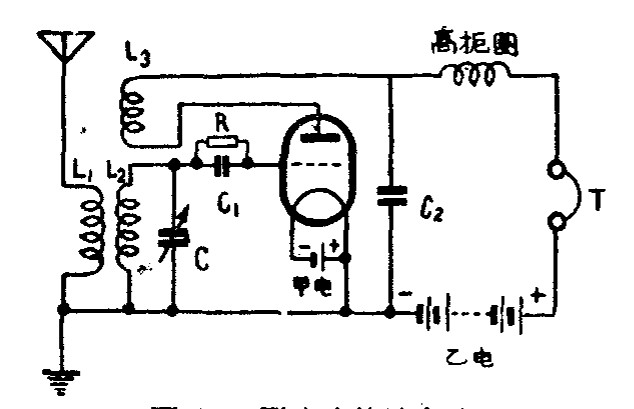
\includegraphics[width=0.9\linewidth]{regenerative_circuit.jpg}
    \caption{再生式检波电路}
    \label{fig:regenerative_circuit}
\end{figure}

\begin{figure}[htbp]
    \centering
    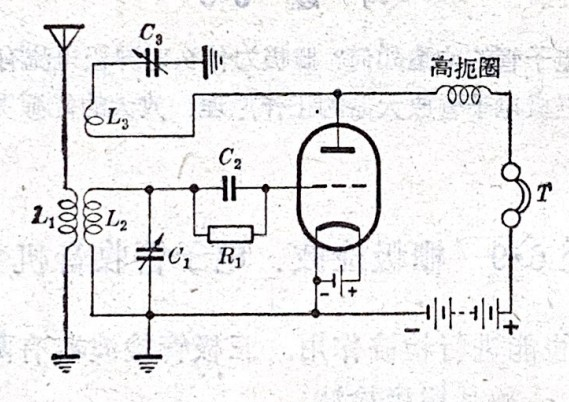
\includegraphics[width=0.9\linewidth]{regenerative_circuit1.jpg}
    \caption{再生式检波电路}
    \label{fig:regenerative_circuit1}
\end{figure}

在图\ref{fig:regenerative_circuit}中，屏极电路的高频扼流线圈（高扼圈）用于防止高频电流流入耳机。高频电流可以通过旁路电容器$C_2$形成回路，从而使再生过程更加稳定。

\section{再生的作用}

再生的主要作用包括：

\begin{enumerate}
    \item \textbf{提高灵敏度}：通过正反馈增强微弱信号，使收音机能够接收更远距离的电台
    \item \textbf{提高选择性}：增强谐振回路的Q值，使调谐更加尖锐
    \item \textbf{增加放大倍数}：反馈信号与输入信号叠加，等效提高了放大能力
\end{enumerate}

\section{再生的控制}

要使再生加大，可以采用以下方法：
\begin{enumerate}
    \item 增加再生线圈$L_3$的圈数；
    \item 缩短$L_2$和$L_3$的距离；
    \item 适当增加屏极电压（不超过规定值）。
\end{enumerate}

再生过强会导致收音机产生振荡电流的啸叫声，不仅无法正常收听，还会从天线上发射出电磁波，干扰附近收音机在相近频带的接收。因此，再生必须加以控制。

收音时，将再生调到将要发生振荡的临界点，此时灵敏度和选择性最佳，声音也最清晰宏亮，这一点称为再生的"临界点"。

再生程度需要适当控制：

\begin{description}
    \item[弱再生] 再生不足，灵敏度提升有限
    \item[临界再生] 接近振荡点，灵敏度和选择性最佳
    \item[强再生] 进入振荡状态，产生自激干扰
\end{description}

通常使用零件节省而效率较高的控制再生的方法有以下几种，各有优缺点：

\subsection{机械调节法}

通过机械变动再生线圈和调谐线圈的距离来控制再生。此法比较简单，但不够稳定，现在很少采用。

\subsection{可变电容器法}

使用可变电容器来控制再生，是最被广泛采用的方法。这是因为它的调谐细致，且可变电容器的机械性能很耐用。

\section{串连式再生与并联式再生}

根据再生线圈连接方式的不同，再生电路主要分为两种类型：

\subsection{串连式再生}

图\ref{fig:series_shunt_regeneration}甲的电路称为"串连式再生"。再生线圈$L_3$串联在屏极电路内，控制再生的可变电容器$C_2$并联在再生线圈的末端和电路零点间。残余高频经过$L_3$后，受到高频扼流圈的阻碍，从$C_2$通过；这样，增减$C_2$的电容量，就能控制通过$L_3$的高频电流，从而使再生受到控制。$C_2$通常称为"再生电容器"。

串连式再生电路的特点是：高频扼流圈有时可以省去不用（因为耳机里的线圈对高频电流也有扼流作用），但是$C_2$的容量要用得大一点，通常是0.00035微法。

\subsection{并联式再生}

图\ref{fig:series_shunt_regeneration}乙是"并联式再生"，再生线圈$L_3$和屏极电路并联；残余高频电流经过$L_3$和$C_2$自成一个回路，受到$C_2$的控制；音频电流则经由高扼圈和耳机等完成回路。因为高扼圈的接入，可以使高频和音频两种电流顺利分路。

并联式再生电路的特点是：$C_2$的电容量可以用得小一点，通常是0.0001微法；高扼圈如果省去，再生力就不够稳定。

\begin{figure}[htbp]
    \centering
    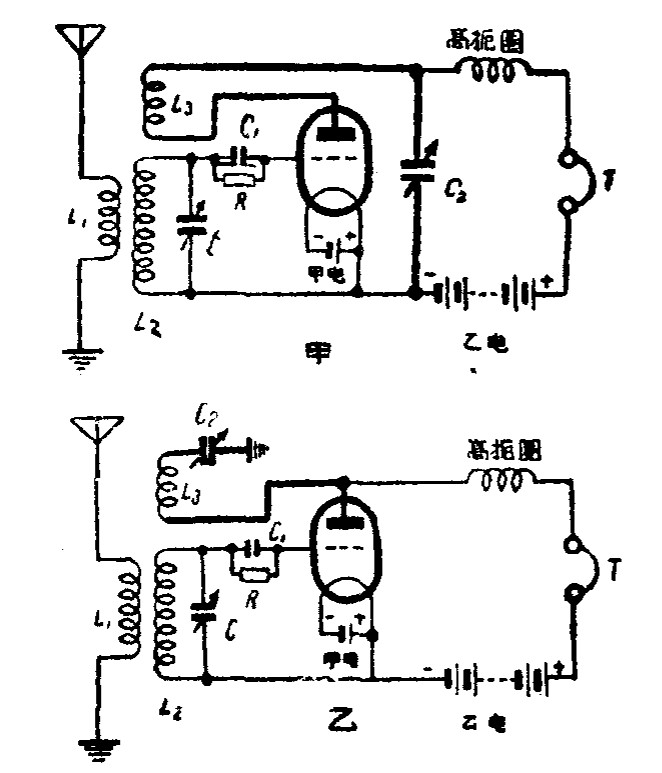
\includegraphics[width=0.9\linewidth]{series_shunt_regeneration.jpg}
    \caption{串连式再生（甲）与并联式再生（乙）电路}
    \label{fig:series_shunt_regeneration}
\end{figure}

\subsection{变动电源电压控制再生}

变动电源电压也可以控制再生。图\ref{fig:voltage_regeneration}就是这样的电路：屏极从并联在乙电上的电位器$R_1$取得可以变动的电压；电压高低就可以增减再生程度。这种方法实际上是通过控制电子管内部的电子流来影响再生的，所以效率也很好。$R_1$的阻值约为50千欧——100千欧，因为在它上面经常有电流通过，所以需要优良质量的电位器，否则很容易烧毁。

\begin{figure}[htbp]
    \centering
    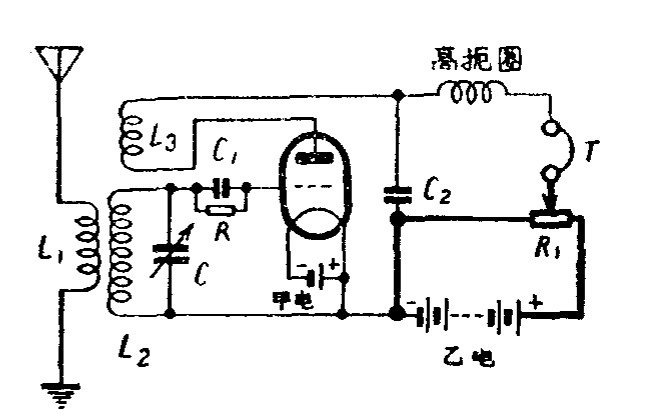
\includegraphics[width=0.7\linewidth]{voltage_regeneration.jpg}
    \caption{变动电源电压控制再生电路}
    \label{fig:voltage_regeneration}
\end{figure}

\subsection{帘栅电压控制再生}

用帘栅电子管作检波工作时，变动帘栅电压来控制管内的电子流，就能更有效地控制再生力。图\ref{fig:screen_grid_regeneration}就是这种电路的装置。将一只电位器$R_1$接入帘栅通向电源的电路上，固定电阻$R_2$是为了防止$R_1$旋到尽头时，避免帘栅受到过高的电压而设，有时可以省掉。当变动$R_1$的阻值时，帘栅上就有不同的电压，使电子流随着增减，再生便受到控制了。$C_3$是帘栅的旁路电容器，使帘栅上的交流成份从它那里流回阴极，不致在帘栅电路里引起交流电压降，影响收音质量，同时对帘栅电压起着稳定作用。

\begin{figure}[htbp]
    \centering
    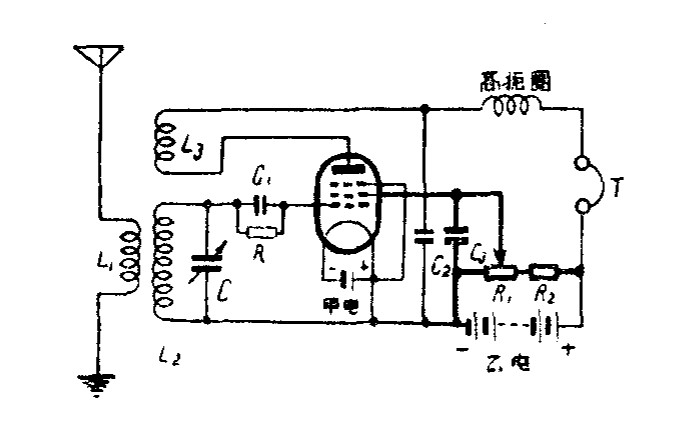
\includegraphics[width=0.9\linewidth]{screen_grid_regeneration.jpg}
    \caption{帘栅电压控制再生电路}
    \label{fig:screen_grid_regeneration}
\end{figure}

一般使用时，$R_1$的阻值常用50千欧，$R_2$为20-50千欧，$C_3$是0.05微法。

这样控制再生的方法非常平稳，效率可算优良，很受人们喜欢。

上面两种电路（变动电源电压控制和帘栅电压控制），再生圈也可以接成并联再生式。

\subsection{电位器并联控制再生}

将电位器并联在再生线圈的两端，使高频电流有一部分从它上面通过。变动电位器时，再生线圈里的电流也将受到影响；这样控制再生的方法也比较平稳。$R_1$的阻值通常是10千欧（图\ref{fig:potentiometer_shunt_regeneration}）。

\begin{figure}[htbp]
    \centering
    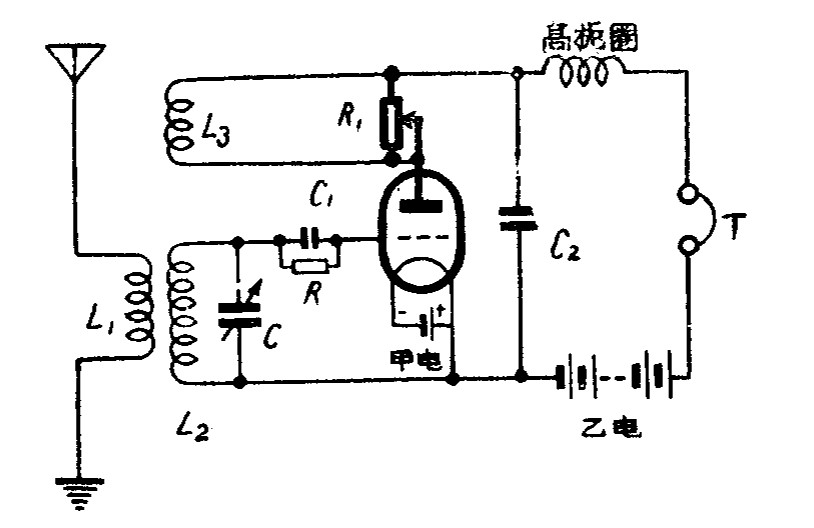
\includegraphics[width=0.7\linewidth]{potentiometer_shunt_regeneration.jpg}
    \caption{电位器并联控制再生电路}
    \label{fig:potentiometer_shunt_regeneration}
\end{figure}

\section{阴极交通再生式电路}

上面介绍的各种再生式电路的共同点，就是它们的再生线圈都是接在屏极电路的输出端的。既然阴极上也通过整个屏流，所以流回阴极一端的电子流也能引起再生，利用这一部分电流而产生再生的，称为阴极交通式（图\ref{fig:cathode_regeneration}）。

\begin{figure}[htbp]
    \centering
    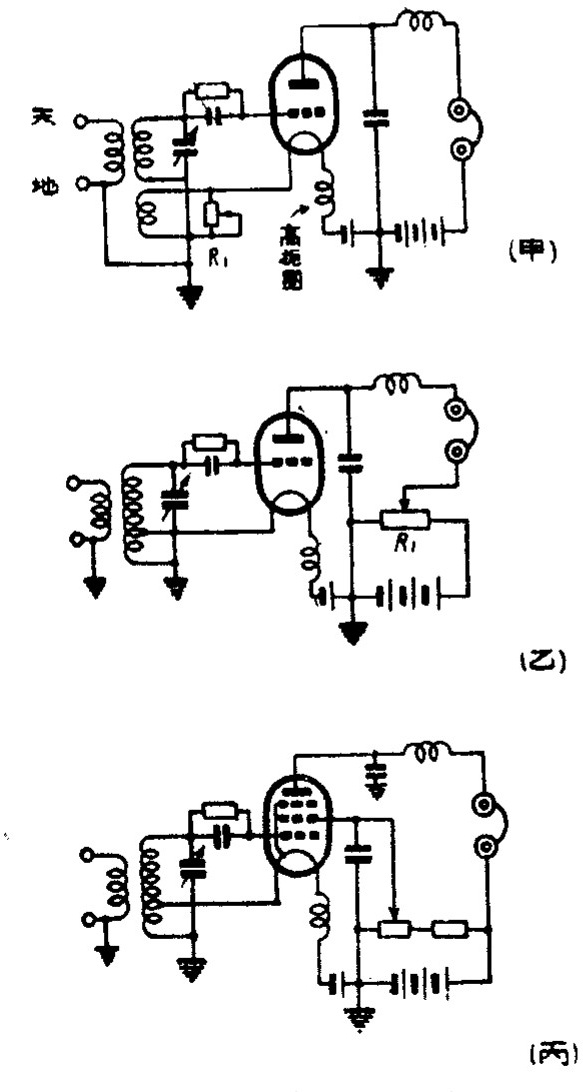
\includegraphics[width=0.8\linewidth]{cathode_regeneration.jpg}
    \caption{阴极交通再生式电路}
    \label{fig:cathode_regeneration}
\end{figure}

阴极交通再生式电路有两种常见接法：一种是将再生线圈接于阴极的一端，为使高频电流完全经过再生线圈，在灯丝的另一脚上接一高频扼流圈，再生控制则利用电阻 $R_1$；另一种是在调谐线圈下面相当圈数处抽一头，接到阴极的一端，当屏极电路的残余高频成份通过这部分时，也能在栅极电路内产生感应电压，这种接法的再生很稳定，且"再生圈"不会因反接而失效。

这种再生方式在电池式收音机中多不采用，因为在灯丝电路中需多用一个高频扼流圈，而性能并未提高。

\section{高频扼流圈}

在屏极电路里，在耳机前面串联一只高频扼流圈，可以阻止残余高频电流流经耳机，并且能够使再生稳定和避免后面所说的"人体感应"。成品的高频扼流圈多绕成蜂房式（图\ref{fig:rf_choke_coil}甲）和分段蜂房式（图\ref{fig:rf_choke_coil}乙）。电感量有2.5毫亨、4.5毫亨和10毫亨等，广播波段收音机里常用后两种。

\begin{figure}[htbp]
    \centering
    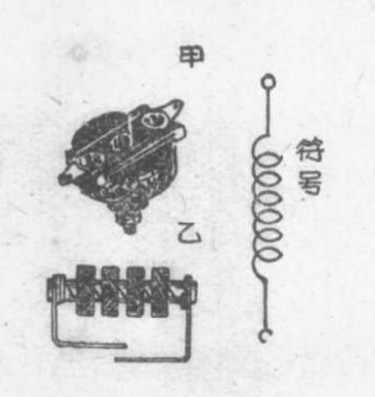
\includegraphics[width=0.9\linewidth]{rf_choke_coil.jpg}
    \caption{高频扼流圈（甲：蜂房式；乙：分段蜂房式）}
    \label{fig:rf_choke_coil}
\end{figure}

高频扼流圈可以自制：用硬纸依尺寸做成线圈盒心子，以直径0.1-0.15毫米的漆包线在上面"乱叠绕"，直到将盒子绕满为止。两个线头分别焊在铆在圆板的两块小焊片（或小铜片）上，外部最好还包一两层纸作为保护（图\ref{fig:homemade_rf_choke}）。

\begin{figure}[htbp]
    \centering
    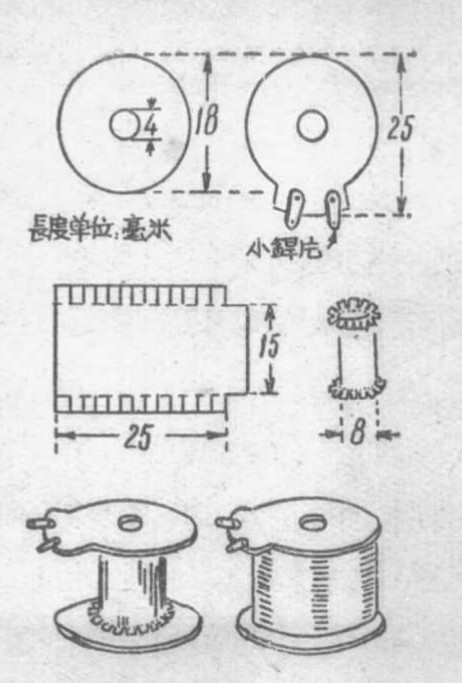
\includegraphics[width=0.7\linewidth]{homemade_rf_choke.jpg}
    \caption{自制高频扼流圈}
    \label{fig:homemade_rf_choke}
\end{figure}

所谓乱叠绕，就是不依排线次序，很不整齐的缠绕；这样绕法可以避免并绕时所产生的线与线之间的"潜布电容量"，使高频电流不能借电容作用通过线圈，提高扼制交流电的作用。乱叠绕和蜂房式的绕法，目的都是为了减少分布电容，其他一些线圈的制作也经常采用这样的绕法。

\section{抽头式（三点式）再生电路}

阴极交通再生式电路的优点在于线圈简单、方向不会弄错。这同样的优点也可以应用于屏极再生电路中，只需将屏极再生电路中的电容与再生线圈位置互换，并把线圈合并即可。这种再生式没有特别的名称，为与普通式加以区别，称为"抽头式"或"三点式"（因为线圈有三个连接点）。进一步简化，可以在调谐线圈中抽出一个头作为天线接头，连天线线圈也省掉了。

\begin{figure}[htbp]
    \centering
    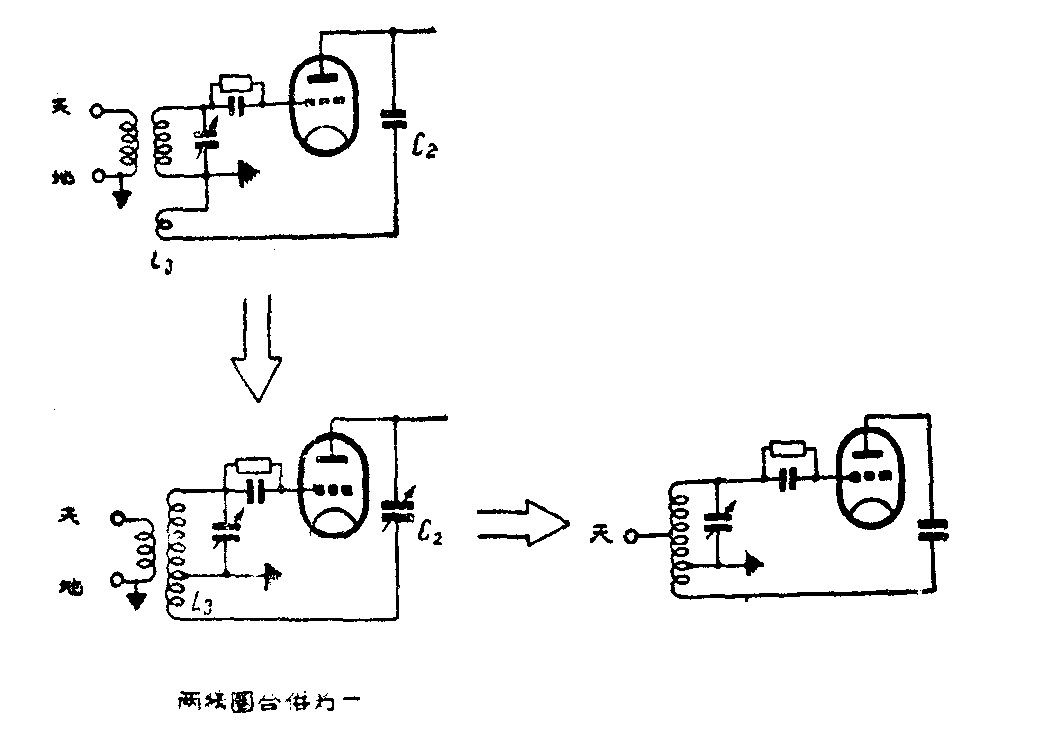
\includegraphics[width=0.8\linewidth]{tapped_regeneration.jpg}
    \caption{抽头式（三点式）再生电路}
    \label{fig:tapped_regeneration}
\end{figure}

\chapter{单管收音机的各种零件}

单管收音机的各种零件，有许多和矿石收音机所用的相同，但也使用一些比较复杂的零件。小部分可以自己制作。

\section{电子管的管座}

电子管的各电极与电路的连接，是通过插入与之匹配的"管座"实现的。管座内有弹簧触点将管脚夹紧，外部接线焊接在弹簧另一端的焊脚上。如果栅极从管顶引出，则需要使用"栅帽"，接线直接焊在栅帽上。

管座主要有两种安装方式：安装在底板上方的"板上式"，特别适用于木质机壳；另一种是目前主流的"板下式"，安装在底板下方，使用更简洁，现代电子管普遍采用这种方式。

每一种名称的电子管都有适合它的管座。有许多电子管的管座是相同的。

每一种名称的电子管，都可以在"电子管特性表"或同类的参考材料上找到它的管座接线图，这是表明电子管的各个电极引线在管座上的位置，以便制作者焊接。它的看法和实际接线时都是把管座翻过来看的，（因为装修收音机时，都是把机座翻过来工作的。）因此绘出来的管座图都是从电子管底部向上看去的"仰视图"。以后我们所用的管座图也都这样绘制。本书所用的电子管，都在图中注出各极接线的位置。

\begin{figure}[htbp]
    \centering
    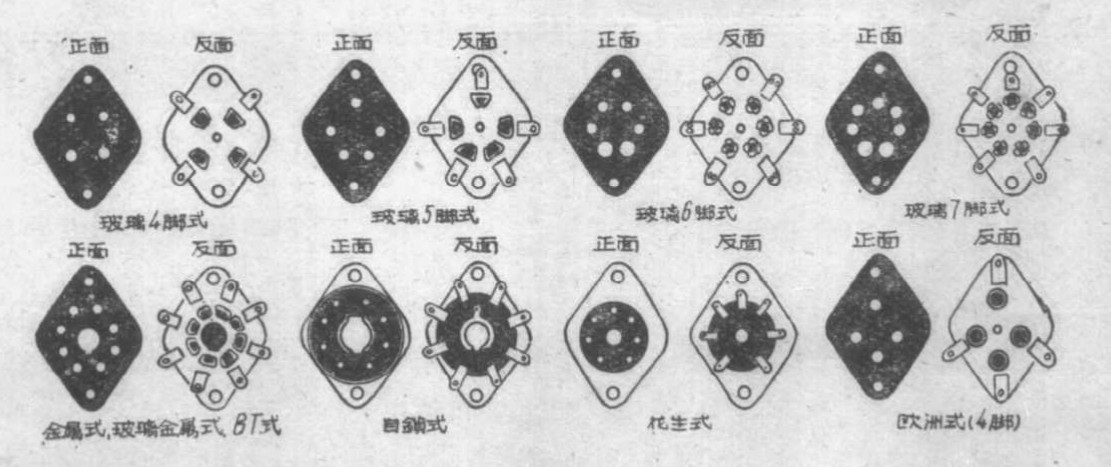
\includegraphics[width=0.8\linewidth]{tube_socket_types.jpg}
    \caption{我国流行的各种类型收音电子管的管座}
    \label{fig:tube_socket_types}
\end{figure}

\section{电子管的管脚类型}

玻璃式电子管的管脚数目随电极数量分为：4脚式、5脚式、6脚式、7脚式等四种。除5脚式外，都有两只脚较粗，即为灯丝引脚；插入电子管时，先找到它们作为定位标准。5脚式管脚间距不同，不易插错。

金属式、玻璃金属式和GT式都使用统一的8脚管座，管脚排列成圆周形，中心有定位键槽。使用时将电子管的定位键对准管座的小缺口，即可正确插入。8脚管座的插孔和电子管脚都编有号码，从小缺口左方起为1，顺时针方向数到8（仰视图视角）。

自锁管的管座也是8脚式，但管脚直径较小，中心有弹性金属筒作为定位键槽，能将定位键"锁"住防止脱落。插脚同样编号为1至8。

花生管采用小7脚插座，无定位键，管脚直径较小，排成大半圆形，圆周上留有一个空位作为识别标记。管脚编号从空位左侧开始为1，依次排到7，1和7的距离最大。

特殊型式的管座也不少，例如老式苏联玻璃四脚管的管座，管脚排成菱形，无大小脚之分，我国无线电爱好者称之为"欧洲式管座"，因其在欧洲大陆最为流行。

\section{电子管的电源}

电子管工作时需要消耗电能，电能的来源称为"电源"。本书各种电路的电源均采用干电池供给。

单管收音机所用的电池分为两组：点燃灯丝的"甲电池"和供给屏极电压的"乙电池"；所有这些电池组都由干电池串联组成。

每个单节干电池的开路端电压约为1.5伏特，电量大小取决于电池的质量和体积，体积大的电池含有的化学物质较多，电量也较强，使用寿命更长。

电池的容量以"安培小时"（Ah）计算，知道了容量，便可以计算出这个电池在收音机里能使用的时间：设电子管需要的电流为$I$（安培），电池容量为$AH$（安培小时），那么可使用的时间$T$（小时）为：

\[ T = \frac{AH}{I} \]

\subsection{国产干电池的种类}

国产干电池在市上出售的有下列五种：

(1) \textbf{甲号电池}（相当于现代大型蓄电池或组合电池组）：容量最大，有20-30安培小时，磁石电话机和多管电池收音机的甲电池多使用它。

(2) \textbf{大号电池}（约相当于现代1号电池）：就是普通手电筒里的电池，容量约2.5安培小时；单管机的甲、乙电和多管电池收音机的乙电适用。

(3) \textbf{3号电池}：是小型手电筒的电池，容量较小，只有2安培小时。可作小型电池式收音机的乙电。

(4) \textbf{4号电池}：较3号略小，容量很小，在0.5安培小时左右，只能作一、二管电池收音机的乙电。

(5) \textbf{5号电池}（约相当于现代7号电池AAA，注意与现代5号电池AA不同，现代AA电池容量通常为1000-2500mAh）：是钢笔电筒里的电池，体积最小，性能和用法同4号电池。

\textit{说明：现代常用的电池型号为1号（大号）、2号、5号（AA）、7号（AAA）等，与本文描述的旧型号体系有所区别。}

\section{电阻器}

电阻器在收音机中的作用是降低（或获取）电路中的电压，或是分流一部分电流。阻值固定的称为"固定电阻"，阻值可调节的称为"可变电阻"。无线电技术中常使用多种不同阻值的电阻，其材质大多为碳膜或金属膜，少数采用电阻丝绕制。

国产碳质固定电阻通过色环表示阻值（单管机所用电阻不多，色环辨认方法本书暂不涉及，购买时说明阻值即可），部分进口电阻则直接在表面印上阻值数字。

可变电阻有两个接线端，一个连接滑动触点，另一个连接电阻体一端。转动旋钮改变触点位置，电路中的电阻值随之变化。国产可变电阻多为胶木外壳，常见阻值有：30欧、20欧、15欧、12欧、6欧等，常用于灯丝电路降压。

电位器是一种特殊的可变电阻，有三个接线端。电阻体两端接电源，转动旋钮时，可在滑动触点上获得连续变化的电位。

国产电位器多数附带电源开关，这是为了安装方便，两者功能相互独立。常见阻值有：10千欧、50千欧、100千欧、250千欧、500千欧和1兆欧等。

\section{电容器}

单管收音机调谐电路里的可变电容器，和矿石收音机所用的完全相同。

固定电容器，本书只使用了种类不多的纸质或云母绝缘的。电容量大小，在零件身上都有注明。

再生力如果是用可变电容器控制的，就需要配置再生电容器。它的电容量，通常是0.0001微法（100皮法），国产产品有很多种类的空气绝缘或纸质绝缘的小型可变电容器（图\ref{fig:variable_capacitor}）。在一些特别的条件下，需要使用较大电容量的可变电容器来控制再生力时，用于调谐电路里的各型可变电容器，只要电容量相同，也一样能使用。

\begin{figure}[htbp]
    \centering
    %\includegraphics[width=0.6\linewidth]{variable_capacitor.jpg}
    \caption{再生可变电容器}
    \label{fig:variable_capacitor}
\end{figure}

有时也要使用"微调电容器"（图\ref{fig:trim_capacitor}）。它的电容量很小，适用于天线和调谐电路的耦合，或者某电路里需要变动微小的电容量来作调谐的时候，常用到它。它的固定片铆牢在胶板上，活动片是一块铜弹片，有螺丝穿着，活动片和固定片间隔以云母。将螺丝旋松旋紧，就能变更弹片间的距离，因而改变了电容量。双连可变电容器里每组附有的补偿电容器就属于这一类。

\begin{figure}[htbp]
    \centering
    %\includegraphics[width=0.5\linewidth]{trim_capacitor.jpg}
    \caption{微调电容器}
    \label{fig:trim_capacitor}
\end{figure}

\section{线圈和它的绕制}

单管收音机和矿石收音机的调谐电路基本相同。但单管机灵敏度更高，对天线多采用松耦合方式以提高选择性。同时，线圈直径可以适当减小，使整机体积更小巧。

再生式电路的再生线圈、初级线圈（即天线线圈）和次级线圈（即调谐电路中的线圈），合称为"三回路线圈"。绕制时，三个线圈的绕向必须相同以确保正确的相位关系。

图\ref{fig:regenerative_coils}是各种通用的再生式电路的线圈，绕制方法列举于后（这里的线圈是与0.00036微法左右的可变电容器相配合的）：

\begin{figure}[htbp]
    \centering
    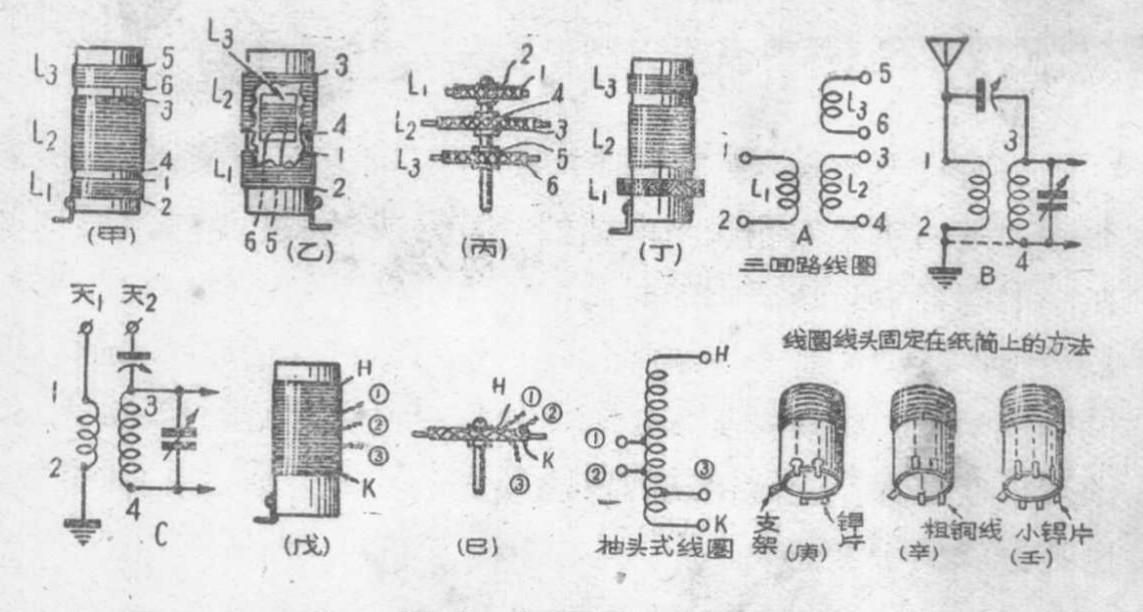
\includegraphics[width=0.9\linewidth]{regenerative_coils.jpg}
    \caption{各种再生式线圈}
    \label{fig:regenerative_coils}
\end{figure}

(1) \textbf{圆筒式}：圆筒直径30毫米，长约80毫米，用直径0.31毫米的漆包线绕制：$L_1$绕35圈，距离5毫米处绕100圈作$L_2$，距$L_2$ 5毫米处绕60圈作$L_3$。

(2) \textbf{双圆筒式}：$L_1$和$L_2$的数据同上，$L_3$直径25毫米，用同号线绕60圈套入$L_2$内，用螺丝固定在外面的大圆筒上，套入前最好先包上一、两层蜡纸，防止碰线。

(3) \textbf{蛛网式}：用直径0.44毫米的线，$L_1$绕30圈，$L_2$绕65圈，$L_3$绕45圈（$L_2$的蛛网板内径为30毫米，其余的是25毫米）。$L_1$和$L_2$的距离约5毫米，$L_2$和$L_3$的距离约10毫米，收音时，还需要依实际情形略为变动。

(4) \textbf{售品线圈}：它的初级线圈是"蜂房式"的，绕线很多——又叫"高总阻式"，设计得当时，可使整个接收范围得到比较均匀的灵敏度，并且可以避免"哑点"。

(5) \textbf{抽头式再生线圈（圆筒式）}：圆筒直径30毫米，用直径0.31毫米的线，从$H$起，绕到第70圈抽头为①，第80圈抽头为②，第100圈抽头为③，继续绕下去到第130圈为止，尾线就是$K$。

(6) \textbf{抽头式再生线圈（蛛网式）}：在大型蛛网板上，用直径0.31毫米的线，从$H$起，绕到第40圈抽头为①，第60圈抽头为②，第70圈抽头为③，继续绕到第95圈为止，尾线是$K$。

为了坚固耐用，各线圈的引线和抽头等，都应该从圆筒里面引出，最好还用焊片、小鞋扣等按数目打在圆筒下部，将各线头焊上，并将它们编好号次，依序排列。简便点，用粗铜线或小铜片穿过纸筒固定起来，也可代替焊片。

自制的线圈，初级多是圈数不多的"低总阻式"。这种线圈对于接收1000千周以上的电波，效率很好；但在接近550千周一段，灵敏度不够，声音会小一点，此时只能换用"高总阻式"线圈。

高总阻式线圈接收近550千周一段的电波效果很好，但有时在接收近1500千周一段的电台时灵敏度不够，补救的方法是在天线和调谐电路之间加入一个微调电容器，对1500千周一段的灵敏度就可以提高。但这样会使1500千周左右的频带被截去一些，应按实际情形将微调电容器略为调整。为了兼顾选择性，可用两个接线柱分别接出，天线接天$_1$处选择性较好，接天$_2$处灵敏度较高。

\chapter{天线回路的耦合方法}

将天线接收的电能量传送给调谐电路的方法，称为\textbf{耦合}。耦合是电路中普遍存在的现象，泛指电能从一部分传递到另一部分的过程。耦合的方式和程度，对收音机的选择性和灵敏度有决定性的影响。

矿石收音机为获得较大音量，常采用直接耦合方式，但这样会使收音机的选择性变差，仅适用于当地电台数量较少的环境。要改善直接耦合的选择性，需要适当减弱天线与调谐电路之间的耦合程度。在天线与调谐电路间串联电容器 C 就是为了这个目的；工作在中波广播波段时，C 可选用电容量为 15-50 皮法(pF)的固定电容器；如使用可变电容器，效果更好，因为可以灵活调节耦合程度。

\begin{figure}[htbp]
    \centering
    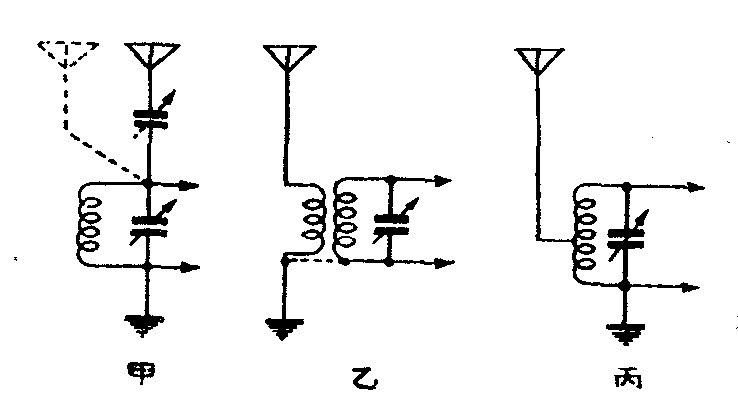
\includegraphics[width=0.8\linewidth]{antenna_coupling.jpg}
    \caption{天线回路的耦合方法}
    \label{fig:antenna_coupling}
\end{figure}

电子管收音机灵敏度较高，大多采用\textbf{电感耦合}（双回路式）。在矿石收音机中，这种方式会影响音量，但在具有放大能力的电子管收音机中无需考虑。通过调整初级线圈的圈数和与次级线圈的距离，可以适当调节灵敏度和选择性，适用于各种不同的收音环境。调谐电路可以接到地线，避免人体对调谐电路的影响。

在调谐线圈近地的一端抽头，作为与天线的\textbf{自耦耦合}，效率良好且线圈绕制简单。抽头越靠近栅极，耦合越紧密（接到顶端则相当于直接耦合）。通常抽出一两个不同圈数的抽头，以便改变耦合程度。

天线线圈和再生线圈的作用虽不相同，但在绕制圈数和距离的处理上常常很相似。

选择天线回路耦合方法的基本原则是：附近电台多时，耦合要松（耦合程度浅或弱），以免相互干扰；附近电台少时，可采用紧耦合。

\chapter{术语表}

\begin{description}
    \item[矿石检波器] 早期无线电接收装置中使用的检测器件
    \item[热电子发射] 金属被加热到炽热状态时表面释放电子的现象，也称爱迪生效应
    \item[真空二极管] 基于热电子发射原理制成的具有单向导电性的电子器件
    \item[直热式阴极] 灯丝本身直接发射电子的阴极结构
    \item[旁热式阴极] 灯丝加热、氧化物阴极发射电子的分离式阴极结构
    \item[单向导电性] 电流只能单向流动的特性
    \item[弗莱明阀] 弗莱明发明的真空二极管
    \item[控制栅极] 位于三极管阴极和阳极之间的金属丝网电极
    \item[真空三极管] 具有放大功能的真空电子器件
\end{description}

\backmatter

\begin{thebibliography}{99}
\addcontentsline{toc}{chapter}{参考文献}
\item 冯报本 编著. 单管收音机[M]. 北京: 人民邮电出版社, 1957.
\item 冯报本 编著. 二、三管收音机[M]. 北京: 人民邮电出版社, 1957.
\end{thebibliography}

\end{document}